% !Mode:: "TeX:UTF-8"
% !TEX program  = xelatex

%\documentclass{cumcmthesis}
\documentclass[withoutpreface,bwprint]{cumcmthesis} %去掉封面与编号页
\usepackage[framemethod=TikZ]{mdframed}
\usepackage{url}   % 网页链接
\usepackage{subcaption} % 子标题
\title{基于多目标优化的高压油管供油与喷油策略设计仿真模型}
\tihao{A}
\baominghao{12006}
\schoolname{合肥工业大学}
\membera{殷振豪}
\memberb{张文钧}
\memberc{徐浩翔}
\supervisor{张莉}
\yearinput{2019}
\monthinput{09}
\dayinput{15}

\begin{document}

 \maketitle
 \begin{abstract}

对高压油管内部燃油的密度和压力进行研究,有助于提高发动机工作的稳定性,对提高发动机的工作效率具有重要的意义。本文根据发动机工作时,燃油的压力变化量和密度变化量之间的比例关系,列出微分方程并进行求解,并利用最优目标规划法,合理规划出最优的高压油管的供油和喷油策略。

\textbf{对于问题一},首先根据燃油的压力变化量和密度变化量之间的比例关系式,列解全微分方程,得到燃油压力和密度之间的关系式。由高压油管的实际工作特性,建立高压油管内燃油的密度和压力随时间变化的仿真模型。写出高压油管燃油进出的流量随时间变化的关系式,并带入到建立的仿真模型中,计算得出燃油密度和压力随时间变化的关系式。利用最优目标规划法,设立优化目标,并用变步长搜索法搜索出最优的策略解。结果为:单向阀开启时长为0.289 ms时,系统压力维持在100 MPa左右;能使压力分别在2s、5s、10s内从100 MPa增长到150 MPa的单向阀开启时长为0.864 ms、0.71 ms和0.71 ms。高压油管的压力达到150 MPa后,将单向阀开启时长调整为0.71 ms便可以一直保持稳定。

\textbf{对于问题二},根据高压油泵和喷油嘴的实际工作规律,重新建立新的进出高压油管的流量随时间变化的关系式,将问题二得到的关系式代回到问题一已经建立的高压油管内燃油密度和压力随时间变化的仿真模型中。利用最优目标规划法,设立优化目标,并用变步长搜索法搜索出最优的策略解。结果为:当角速度$\omega=14.15\pi\,$rad/s时,系统的稳定性最佳。

\textbf{对于问题三},首先利用控制变量法,定量地分析只有喷油嘴或只有限压阀时对油管燃油压力的影响,分别得到喷油嘴和限压阀各自的工作特性。对于第一问,我们在保持喷油嘴工作周期不变的基础上,设置不同的喷油嘴开启时间,使得喷油嘴在一个周期内交替工作,利用最优目标规划法得到最优的喷油嘴交替开启时间。当凸轮角速度$\omega=28.34\pi\,$rad/s,喷油嘴B开启时间为1.1 ms、喷油嘴C的开启时间为50.4 ms时,系统的稳定性最佳。对于第二问,充分利用喷油嘴和限压阀各自的工作特性,在一个供油周期内严密计算得到最佳的开启和关闭时间,设计出最佳的高压泵和减压的控制方案,使得在每一周期内高压油管的工作压力能更稳定的控制在100 MPa左右,详细结果见\cref{fig:Q32o}。

\textbf{最后},将模型应用于某老式柴油发动机上,根据该柴油发动机的实际参数,计算出理论数据并与实际数据作比对。客观评价模型的优缺点,并对模型存在的不足提出改进的方向。


\keywords{供喷油方案设计\quad 微分方程\quad   仿真模型\quad  多目标优化}
\end{abstract}

%目录  2019 明确不要目录,我觉得这个规定太好了
%\tableofcontents

%\newpage

\section{问题重述}
\subsection{背景知识}

截止至2018年底,中国人口数量已达13.95亿,在庞大的人口数量背后是极速增长的交通需求和对机动类交通工具的依赖。但从目前我国制造业发展水平来看,发动机的制造工艺仍属于我们亟待解决的重难点问题。中国零部件制造业起步相对较晚,发动机制造的关键技术和尖端技术被发达国家所掌握,因此我国发动机制造企业在技术创新和产品研发方面严重依赖于发达国家,缺乏自主创新能力。由于我国发动机制造受制于制造水平和对发动机原理等的理解程度,我国制造的发动机在持久性、稳定性和其他功能方面远比不上世界第一流的发动机。目前摆在发动机制造企业面前有许多尚未解决的技术,其中一项便是高压油管的压力控制。高压油管的压力控制决定了喷油性能的优劣,进而影响了汽车的燃烧功能、使用寿命等一系列问题,是制造业亟待解决的问题。

\subsection{具体问题}

问题一:某型号高压油管的内腔长度为500 mm,内直径为10 mm,供油入口A处小孔的直径为1.4 mm,通过单向阀开关控制供油时间的长短,单向阀每打开一次后就要关闭10 ms。喷油器每秒工作10次,每次工作时喷油时间为2.4 ms,喷油器工作时从喷油嘴B处向外喷油的速率如\cref{fig:pyslsyt}所示。高压油泵在入口A处提供的压力恒为160 MPa,高压油管内的初始压力为100 MPa。如果要将高压油管内的压力尽可能稳定在100 MPa左右,如何设置单向阀每次开启的时长?如果要将高压油管内的压力从100 MPa增加到150 MPa,且分别经过约2s、5s和10s的调整过程后稳定在150 MPa,单向阀开启的时长应如何调整?

\begin{figure}[!h]
	\centering
	\includegraphics[width=.7\textwidth]{pysl}
	\caption{喷油速率示意图}
	\label{fig:pyslsyt}
\end{figure}

问题二:在实际工作过程中,高压油管A处的燃油来自高压油泵的柱塞腔出口,喷油由喷油嘴的针阀控制。高压油泵柱塞的压油过程如\cref{fig:gyyg}所示,凸轮驱动柱塞上下运动,凸轮边缘曲线与角度的关系见附件1。柱塞向上运动时压缩柱塞腔内的燃油,当柱塞腔内的压力大于高压油管内的压力时,柱塞腔与高压油管连接的单向阀开启,燃油进入高压油管内。柱塞腔内直径为5 mm,柱塞运动到上止点位置时,柱塞腔残余容积为20 mm$^3$。柱塞运动到下止点时,低压燃油会充满柱塞腔(包括残余容积),低压燃油的压力为0.5 MPa。喷油器喷嘴结构如\cref{fig:pyz}所示,针阀直径为2.5 mm、密封座是半角为9°的圆锥,最下端喷孔的直径为1.4 mm。针阀升程为0时,针阀关闭;针阀升程大于0时,针阀开启,燃油向喷孔流动,通过喷孔喷出。在一个喷油周期内针阀升程与时间的关系由附件2给出。在问题1中给出的喷油器工作次数、高压油管尺寸和初始压力下,确定凸轮的角速度,使得高压油管内的压力尽量稳定在100 MPa左右。

\begin{figure}[!h]
	\centering
	\includegraphics[width=.7\textwidth]{gyyg}
	\caption{高压油管实际工作过程示意图}
	\label{fig:gyyg}
\end{figure}

\begin{figure}[!h]
	\centering
	\includegraphics[width=.4\textwidth]{pyz}
	\caption{喷油器喷嘴放大后的示意图}
	\label{fig:pyz}
\end{figure}


问题三:在问题2的基础上,再增加一个喷油嘴,每个喷嘴喷油规律相同,喷油和供油策略应如何调整?为了更有效地控制高压油管的压力,现计划在D处安装一个单向减压阀(\cref{fig:jyf})。单向减压阀出口为直径为1.4 mm的圆,打开后高压油管内的燃油可以在压力下回流到外部低压油路中,从而使得高压油管内燃油的压力减小。请给出高压油泵和减压阀的控制方案。

\begin{figure}[!h]
	\centering
	\includegraphics[width=.7\textwidth]{jyf}
	\caption{具有减压阀和两个喷油嘴时高压油管示意图}
	\label{fig:jyf}
\end{figure}

\textbf{注1.}燃油的压力变化量与密度变化量成正比,比例系数为$\frac{E}{\rho}$,其中$\rho$为燃油的密度,当压力为100 MPa时,燃油的密度为0.850 $\text{mg/mm}^{3}$。$E$为弹性模量,其与压力的关系见附件3。

\textbf{注2.}进出高压油管的流量为$Q=CA\sqrt{\frac{2\Delta P}{\rho}}$,其中$Q$为单位时间流过小孔的燃油量(mm$^{3}$/ms),$C=0.85$为流量系数,$A$为小孔的面积(mm$^{2}$),$\Delta P$为小孔两边的压力差(MPa),$\rho$为高压侧燃油的密度($\text{mg/mm}^{3}$)。


\section{模型的假设及符号说明}
\subsection{模型的假设}
\begin{enumerate}
	\item 高压油管无裂纹,不会破裂。
	\item 燃油在不同压力下始终能充盈容器。
\end{enumerate}

\subsection{符号说明}

% Table generated by Excel2LaTeX from sheet 'Sheet1'
\begin{table}[htbp]
	\centering
	\begin{tabular}{cccc}
		\hline
		\hline		
		符号    & 意义    & 符号    & 意义 \\
		\hline
		\hline
		$P_{0}$ & 高压油管内初始压力 & $\rho_{0}$ & 高压油管内初始液体密度 \\
		$t_{0}$ & 高压油泵打开时长 & $t_{1}$ & 高压油泵打开后关闭时长 \\
		$P_{a}$ & 高压油管内实际压力 & $\rho_{a}$ & 高压油管内实际液体密度 \\
		$Q_{0}$ & 喷油嘴流出流量 & $Q_{i}$ & 高压油泵向油管内的供油量 \\
		$V_{a}$ & 油管体积  & $A_{i}$ & 油泵与油管间的连接孔大小 \\
		$\omega$ & 凸轮转动角速度 & $\theta(t)$ & 凸轮极角 \\
		$V_{t}$ & 高压油泵容积 & $R_{0}$ & 高压油泵柱塞腔半径 \\
		$r_{t}$ & 高压油泵极径 & $r(0)$ & 高压油泵初始极径 \\
		$\widetilde{\rho}$ & 虚燃油密度 & $\widetilde{P}$ & 虚燃油压力 \\
		$\rho(t)$ & 实燃油密度 & $P(t)$ & 实燃油压力 \\
		$A_{0}$ & 漏环面积  & $x(t)$ & 针阀的升程 \\
		$r$   & 针阀底部中心到密封座垂线距离 & $h$   & 针阀底部中心到顶角的距离 \\
		$P_{r}$ & 发动机燃烧室压力 & $G$   & 压力差 \\
		\hline
		\hline
	\end{tabular}%
	\label{tab:fhsm}%
\end{table}%



\section{问题的分析}
\subsection{研究现状的综述}

当前学术界对于高压油管的研究重点在于研究高压油管的形状对喷油和整个发动机的影响。研究燃油喷射系统中高压油管的压力波动问题,有利于提高发动机的稳定性。姜峰\upcite{bib:1}通过仿真实验认为在高压油管长度一定时,高压油管直径越小,喷油器嘴端压力越高,在不同配比生物柴油条件下,由油压压力最高确定高压油管直径为2 mm时,喷油器嘴端压力较稳定;同时在高压油管直径为2 mm时,随着高压油管长度增大,喷油器嘴端压力呈现下降趋势,由不同配比生物柴油出现嘴端压力拐点确定高压油管长度为500 mm,有利于嘴端压力稳定。韩江枫\upcite{bib:2}指出油管固定点和管夹的位置变化、数量增加和油管形状改变均可提高高压油管的各阶固有频率, 其中增加固定点的方法最为明显, 设计者可优先考虑。韩国的Lee\upcite{bib:3}通过实验证明燃油的粘温粘压效应十分明显。苏海峰\upcite{bib:4}通过分析发现随着主预间隔时间的变化,主喷油量会量现周期性波动,且波动的幅度是随着主预间隔的增加而不断衰弱。


\subsection{对问题的具体分析}
\subsubsection{对问题一的具体分析}

根据题目中给出的燃油压力变化量$\Delta P$与密度变化量$\Delta \rho$的比例关系,我们由此列出微分方程并求解,得到燃油压力$P$与密度$\rho$的函数关系式。当单向阀或喷油嘴开启时,油管与其他系统有燃油交换,所以高压油管内燃油的压力$P$和密度$\rho$会随着燃油交换而变化。根据题目中给出的进出高压油管油量的公式,计算出每一时刻高压油管内的燃油压力,利用最优目标规划法,解出使得燃油压力始终稳定在100 MPa的单向阀开启时长;对于在指定时间内增长至150 MPa的情况,迭代计算出每一时刻的燃油压力,并与目标压力比较,得到最符合题意的单向阀开启时长。

\subsubsection{对问题二的具体分析}

在问题一的基础上,问题二中的进出油的规律发生了改变。我们首先根据针阀和高压泵的工作规律,分别建立燃油压力和密度随时间变化模型。再将得到的关系式重新代回到问题一已建立的高压油管的压力随时间变化模型中。迭代计算每一时刻的燃油压力,利用最优目标规划法,与目标压力比较,得到最优的凸轮的角速度。

\subsubsection{对问题三的具体分析}
在问题二的基础上,对于问题一,题目中增加了一个新的喷油孔C,在此基础上,我们寻找更加稳定的供油和喷油方案。为此,我们新增了一个优化目标,用来描述高压油管工作时间内的压力与标准100 MPa之间的最大压力差。并将降低最大压力差为第一优化目标,压力差平方和最小为第二优化目标,并寻找符合优化目标函数的供油和喷油策略;对于第二问,我们首先利用控制变量法来研究喷油嘴和减压阀的工作特性,并结合实际的工作规律,利用最优目标规划法,得到最佳的高压油泵和减压阀的控制方案。

\section{模型的建立及求解}
\subsection{问题一的分析及求解}

首先使用根据附件三所给出的弹性模量与压力的数据对应表,利用MATLAB软件拟合出弹性模量$E$关于压力$P$的函数关系式。

\begin{equation}
\ln E=0.0039P+7.31
\label{eq:E-P}
\end{equation}

两边取$e$次幂,可得如下公式
\begin{equation}
E(P)=e^{0.0039P+7.31}
\label{eq:2}
\end{equation}

单位为MPa,相关系数$R^{2}=0.995$,拟合效果极好。
\subsubsection{建立燃油压力P与密度ρ之间的函数关系模型}

因为燃油的压力变化量与密度变化量成正比,比例系数为$\frac{E}{\rho}$,其中$\rho$为燃油的密度。

所以我们列出如下微分关系式
\begin{equation}
dP= \frac{E(P)}{\rho}d\rho
\end{equation}

分离变量得

\begin{equation}
\frac{dP}{E(P)}=\frac{d\rho}{\rho}
\end{equation}

将$E(P)$代入

\begin{equation}
\frac{dP}{e^{0.0039p+7.31}}=\frac{d\rho}{\rho}
\end{equation}

两边取定积分

\begin{equation*}
\int_{P_{0}}^{P}\  \frac{dP}{e^{0.0039P+7.31}} = \int_{\rho_{0}}^{\rho}\ \frac{d\rho}{\rho}
\end{equation*}

取当$P_0=100\,$MPa时,$\rho_0=0.850\,\text{mg/mm}^{3}$

即
\begin{equation}
e^{-0.0039P}=-5.8312\ln{\frac{\rho}{0.85}} +1.47698
\end{equation}

以$\rho$为自变量,$P$为因变量,得到$P$关于$\rho$的函数关系式\cref{eq:P-rho},关系图如\cref{fig:P-rho}所示。
\begin{equation}
P=\frac{1}{-0.0039}\ln{\left[(-5.8312)\ln\frac{\rho}{0.85}+0.677\right]}  
\label{eq:P-rho}
\end{equation}

\begin{figure}[!h]
	\centering
	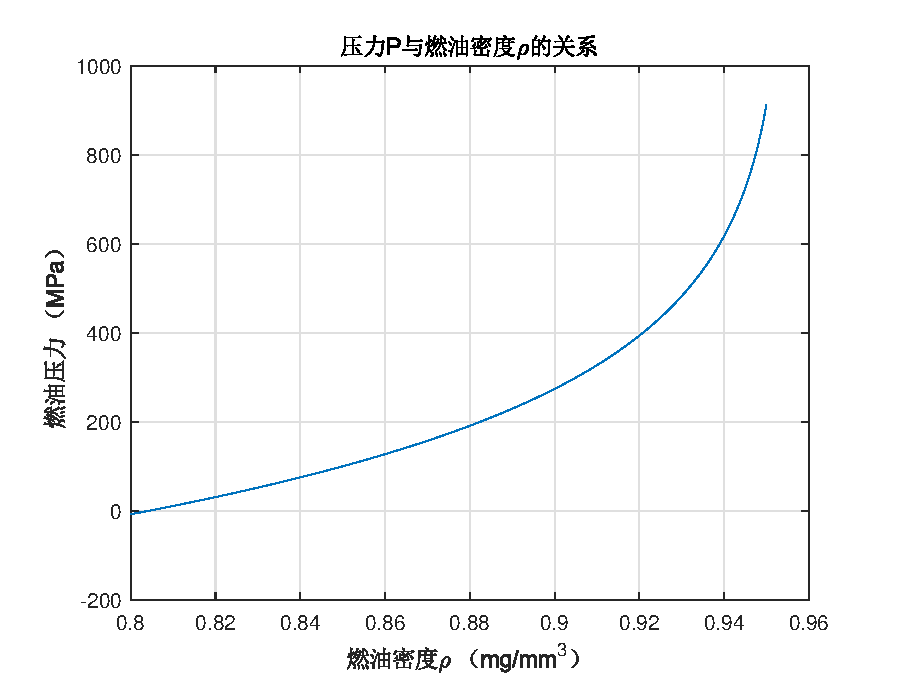
\includegraphics[width=.8\textwidth]{P-rho}
	\caption{压力$P$随燃油密度$\rho$变化图}
	\label{fig:P-rho}
\end{figure}


以$P$为自变量,$\rho$为因变量,得到$\rho$关于$P$的函数关系式\cref{eq:rho-P},关系图如\cref{fig:rho-P}所示。
\begin{equation}
\rho=\exp \left[-0.1715\left(e^{-0.0039P}-0.677\right)+\ln 0.85 \right]
\label{eq:rho-P}
\end{equation}

\clearpage

\begin{figure}[!h]
	\centering
	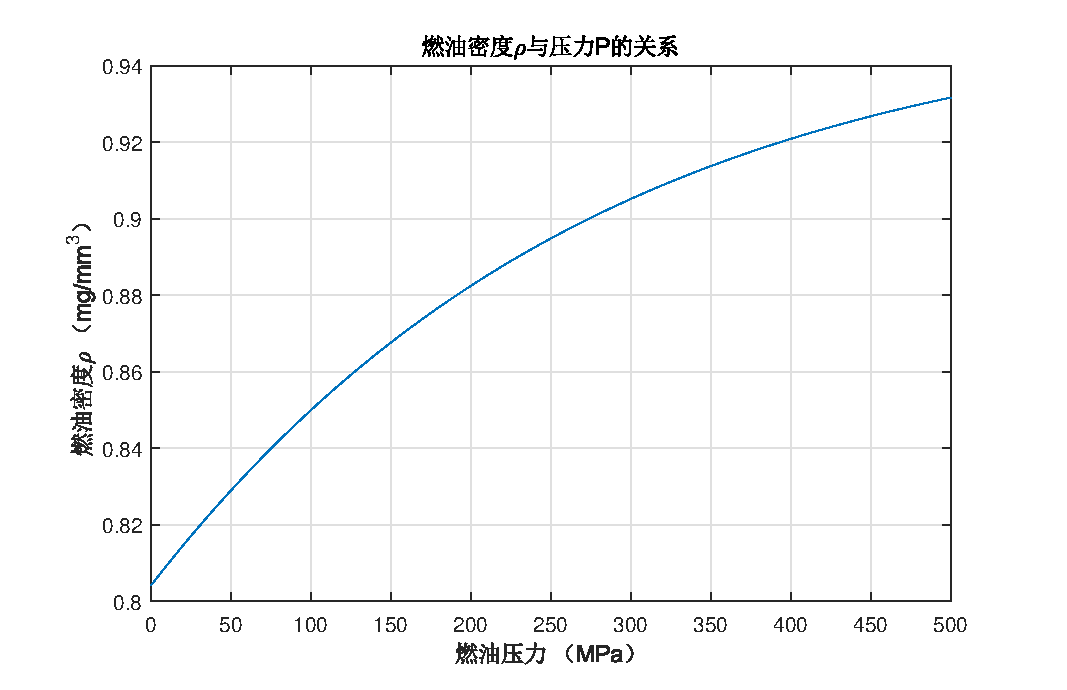
\includegraphics[width=.8\textwidth]{rho-P}
	\caption{燃油密度$\rho$随压力$P$变化}
	\label{fig:rho-P}
\end{figure}



\subsubsection{高压油泵向高压油管内供油的流量函数模型}

根据题意高压油泵这一侧的液体压力恒为160 MPa,所以由上面推导的公式\cref{eq:rho-P}可知高压侧燃油的密度保持恒定且密度为
\[
\rho=\exp\left [-0.1715\left (e^{-0.0039\times160}-0.677 \right )+\ln 0.85\right ]=0.8708\,\text{mg/mm}^{3}
\]

由题中注二可得,进出高压油管的流量公式为:

\begin{equation}
Q=CA\sqrt{\frac{2 \Delta P}{\rho}}
\end{equation}

其中Q为单位时间流过小孔的燃油量(mm$^3$/ms),C=0.85为流量系数,A为小孔的面积(mm$^2$),$\Delta P$为小孔两边的压力差(MPa),$\rho$为高压侧燃油的密度(mg/mm$^3$)。


设高压油泵每次打开的时间为$t_0$,打开后的关闭时间为$t_1$,所以高压油泵的一个供油周期为$T$。

 \begin{equation}
T=t_0+t_1
\label{eq:energy}
\end{equation}

设$\Delta t$为一个时间极短的供油时间间隔,则在每一个工作周期的任意极短供油时间内,由公式\cref{eq:Qi}可得,油泵向油管内部供油的流量大小为 $Q_{i}(t)\cdot \Delta t$。

\begin{equation}\label{eq:Qi}
Q_i(t)\cdot \Delta t =\left\{
\begin{array}{lcr}
    CA_{i}\sqrt{\frac{2\times(160-P_a(t))}{\rho(160)}} \Delta t & & { 0\le t\le t_0}\\
	0 & & {t_0<t<T}
\end{array} \right.
\end{equation}

\subsubsection{喷油嘴喷出的燃油随时间变化模型}

因为喷油器每秒工作10次,则喷油器的一个完整工作周期为100 ms。在每一个喷油工作时期内,喷油速率与时间的关系如\cref{fig:pyslsyt}所示

根据题目中\cref{fig:pyslsyt}曲线所标注的数据,易得一个周期内喷油速率$Q_o$与时间的函数关系式为:

\begin{equation}
Q_o(t)=\left\{
\begin{array}{lcc}
100t & & { 0\le t<0.2}\\
20 & & {0.2\le t\le 2.2}\\
240-100t & & {2.2<t\le 2.4}\\
0 & & {2.4<t\le 100}
\end{array} \right.
 \end{equation}
 
设$\Delta t$为一个时间极短的喷油时间间隔,则在每一个工作周期的任意极短喷油时间内,喷嘴向外喷油的流量大小为$Q_o(t)\cdot \Delta t $
	
	
\subsubsection{高压油管内燃油的密度和压力变化模型}
	
我们假设在一定范围内,高压油管内部的液体是充盈于油管的。即有少量燃油流进或流出后,管内液体会收缩或膨胀并充满整个油管。
%
根据题目中所给的油管内径和油管长度数据,可得油管的体积
\begin{equation}
	V_{a}=\pi r^{2}l	
\end{equation}

在4.1.2节和4.1.3节的模型中我们已经求得关于$Q_i$和$Q_o$关于$t$的函数关系式,再以$Q_i$、$Q_o$为自变量,以此解得油管内部燃油的密度$\rho_{a}$和压力$P_a$随时间变换的微分方程。在$t=0$时,初始条件为$\rho_{a} (t)=0.85,P_{a}(t)=100$,油管中液体在压力为160 MPa时的密度即$\rho_{a}(160)=0.8708$。在此初始条件下,列出油管内部燃油的密度和压力的微分方程如下所示:
\begin{equation} \label{eq:rho_{a}(t)}
\rho_{a}(t)=\rho_{a}(t-\Delta t)+\frac{0.8708\times Q_i(t) -Q_o(t)\rho_{a}(t-\Delta t)}{V_{a}}	\Delta t
\end{equation}
	
\begin{equation} \label{eq:P_{a}(t)}
P_{a}(t)=\frac{1}{-0.0039}\ln \left[\left(-5.8312 \right) \ln \frac{\rho_{a}(t)}{0.85}+0.677\right]
\end{equation}

在已知初始条件的情况下,我们选取足够小的时间间隔$\Delta t$,然后利用微分方程进行仿真模拟实验。通过在初始$t=0$条件下,每次增加$\Delta t$的时间间隔,直至增加到$t=T$即一个喷油周期的时长。模拟递推出在这个喷油周期内,每一时刻油管内部燃油的密度和压力的大小。

为了表达方便,记
\begin{equation}
Z(t)=\frac{0.8708Q_i(t) -Q_o(t)\rho_{a}(t-\Delta t)}{V_{a}}		
\end{equation}

\begin{equation}\notag
\left\{
\begin{align}
\rho(\Delta t) &= \rho(0)+Z(\Delta t)\Delta t \\
\rho(2 \Delta t) &=\rho(\Delta t)+Z(2 \Delta t)\Delta t \\
\cdots & \\
\rho(t-\Delta t) & = \rho(t-2\Delta t)+Z(t-\Delta t)\Delta t
\end{align}
\right.
\end{equation}

如此从初始时刻$t=0$开始,只要取的$\Delta t$足够小,便可以利用迭代法递推任意时刻燃油的压力和密度。如此,我们最终得到的$\rho(t-\Delta t)$就可以无限逼近于表示高压油管密度的连续函数$\breve{\rho} (t)$。

\begin{equation*}
\lim\limits_{\Delta t \rightarrow 0} \rho(t-\Delta t)=\breve{\rho}(t)
\end{equation*}

\subsubsection{最优单向阀开启时长目标优化}

问题一要求我们调整单向阀的开启时长$t_0$,使得高压油管内的压力尽可能稳定在100 MPa左右。在给定某一单向阀开启时长的情况下,通过高压油管的压力变化模型,可以得到任意时刻油管内部的压力。如式\cref{eq:F(i)}将每一时刻计算得到的压力与目标压力$P_a(0)=$100 MPa作差求平方,将每一时刻的平方累加求和得到$F(t)$,并取使$F(t)$取得最小值时的$t$为最优开启时长。

\begin{equation} \label{eq:F(i)}
F(t)=\sum_{n=0}^N[P_a(n\Delta t)-P_a(0)]^2
\end{equation}

\subsubsection{问题一的求解结果}
问题一中的限制条件如下所示
\begin{align}
&Q_i(t)=\left\{
\begin{array}{lcr}
CA\sqrt{\frac{2\times(160-P_a(t))}{\rho(160)}}\Delta t & & { 0\le t\le t_0}\\
0 & & {t_0<t<t_1}
\end{array} \right.\\
&Q_o(t)=\left\{
\begin{array}{lcr}
100t & & { 0\le t<0.2}\\
20 & & {0.2\le t\le 2.2}\\
240-100t & & {2.2<t\le 2.4}\\
0 & & {2.4<t\le 100}
\end{array} \right.
\end{align}

在题目一的限制条件下,由上述公式\cref{eq:rho_{a}(t)}、公式\cref{eq:P_{a}(t)}联立求解

\begin{align}
&\rho_a(t)=\rho_a(t-\Delta t)+\frac{Q_i(t) \rho_a(160) \Delta t-Q_o(t)\rho_a(t-\Delta t)\Delta t}{V}\\
&P_a(t)=\frac{1}{-0.0039}\ln{\left[(-5.8312)\ln\frac{\rho_a(t)}{0.85}+0.677\right]}	
\end{align}

取时间间隔$\Delta t=0.01\,$ms,利用变步长搜索法来对单向阀开启时长进行遍历,并求得每一单向阀所对应的压力差平方和。利用MATLAB软件进行计算,求得当单向阀开启时长$t_0=0.289\,\text{ms}$的时候,油管内部的压力最稳定且保持在100 MPa左右,如\cref{fig:Q1_1}所示:

\begin{figure}[!h]
	\centering
	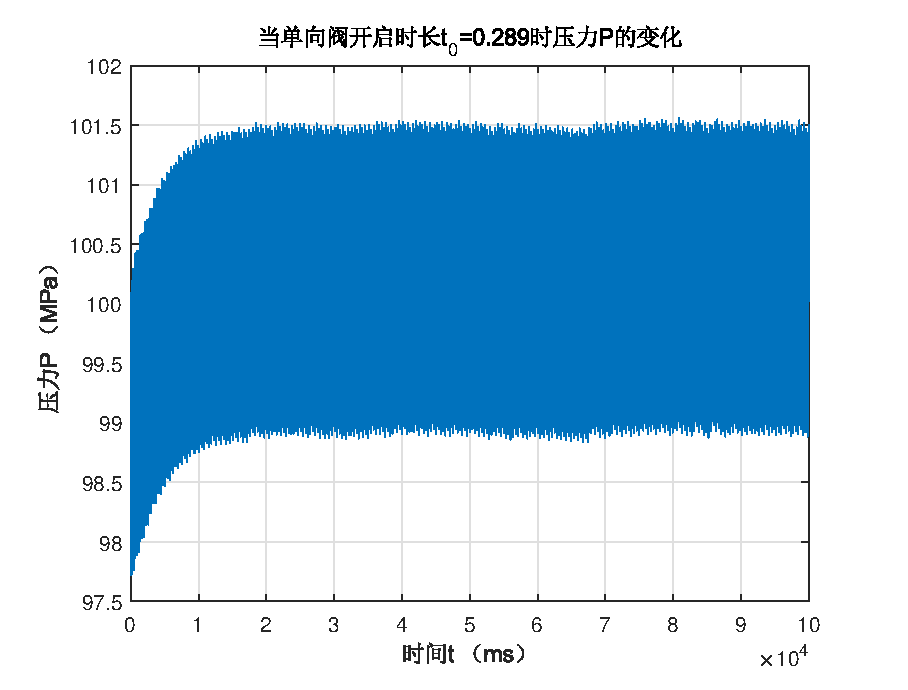
\includegraphics[width=.8\textwidth]{Q1_1}
	\caption{$t_{0}=0.289$时压力$P$变化图}
	\label{fig:Q1_1}
\end{figure}
	
	
	
对于高压油管内的压力经过不同的时间从100 MPa增长到150 MPa的情况,我们分别求解经过2s、5s、10s后的压力与目标压力的压力差平方和,总数值最小的的单向阀开启时间,即为我们的最佳开启时间,利用MATLAB软件计算结果如\cref{tab:wt1}所示,$P(t)$变化图如\cref{fig:Q1_2runto150in2s}、\cref{fig:Q1_2runto150in5s}、\cref{fig:Q1_2runto150in10s}、\cref{fig:Q1_2keep150}。

% Table generated by Excel2LaTeX from sheet 'Sheet1'
\begin{table}[htbp]
	\centering
	\caption{问题1计算结果表}
	\begin{tabular}{ccc}
		\hline
		\hline
		增压时间$t$(s) & 单向阀开启时间(ms) & 第$t$秒时高压油管压力(MPa) \\
		\hline
		\hline
		2     & 0.864 & 149.9937 \\
		5     & 0.71  & 149.9913 \\
		10    & 0.71  & 150.1716 \\
		\hline
		\hline
	\end{tabular}%
	\label{tab:wt1}%
\end{table}%



\begin{figure}[!h]
	\centering
	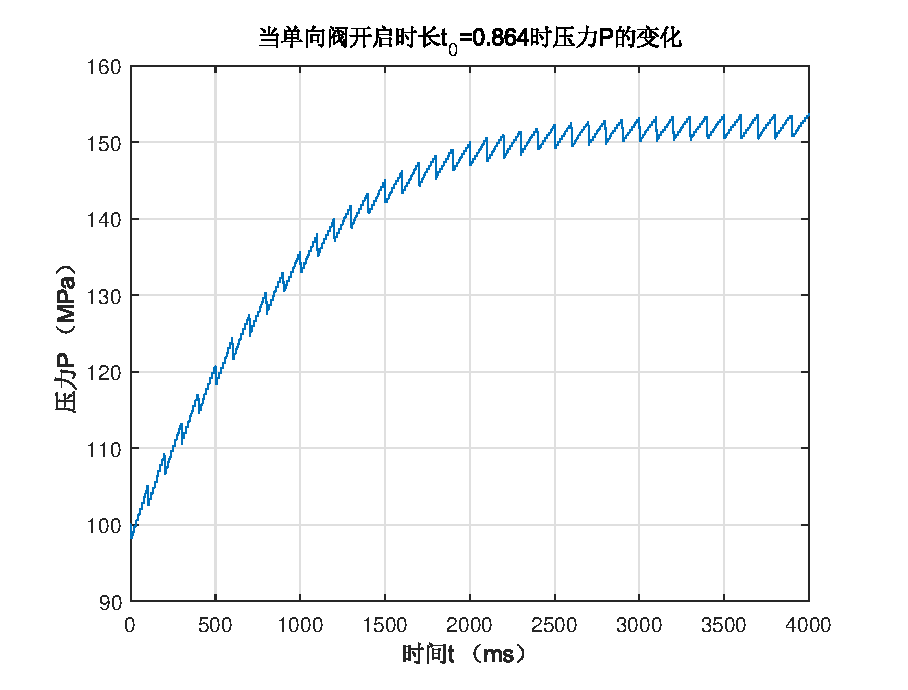
\includegraphics[width=.8\textwidth]{Q1_2runto150in2s}
	\caption{经过2s稳定至150MPa$\,P(t)$图}
	\label{fig:Q1_2runto150in2s}
\end{figure}

\begin{figure}[!h]
	\centering
	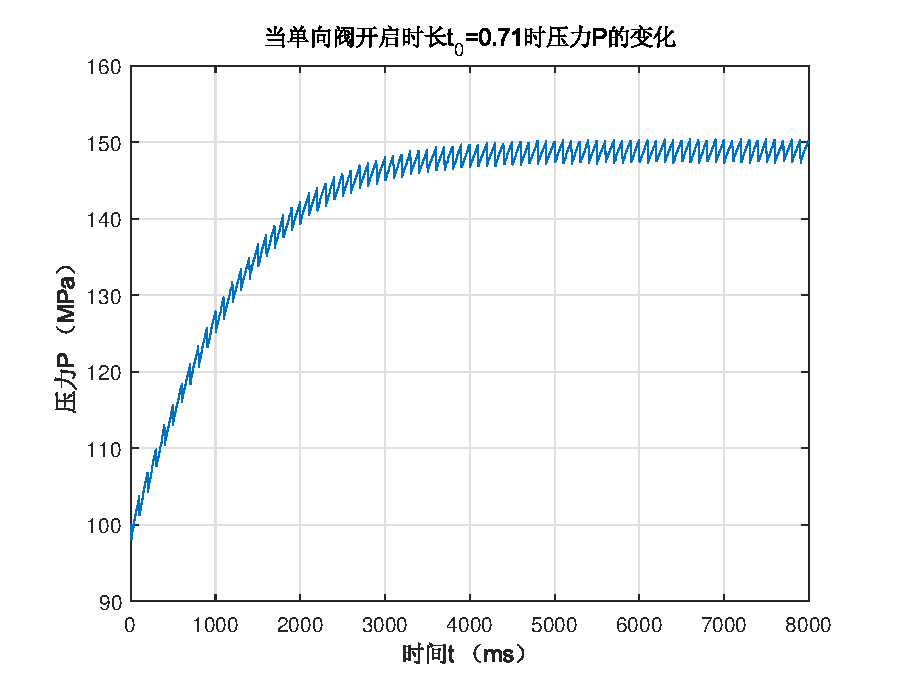
\includegraphics[width=.8\textwidth]{Q1_2runto150in5s}
	\caption{经过5s稳定至150MPa$\,P(t)$图}
	\label{fig:Q1_2runto150in5s}
\end{figure}

\begin{figure}[!h]
	\centering
	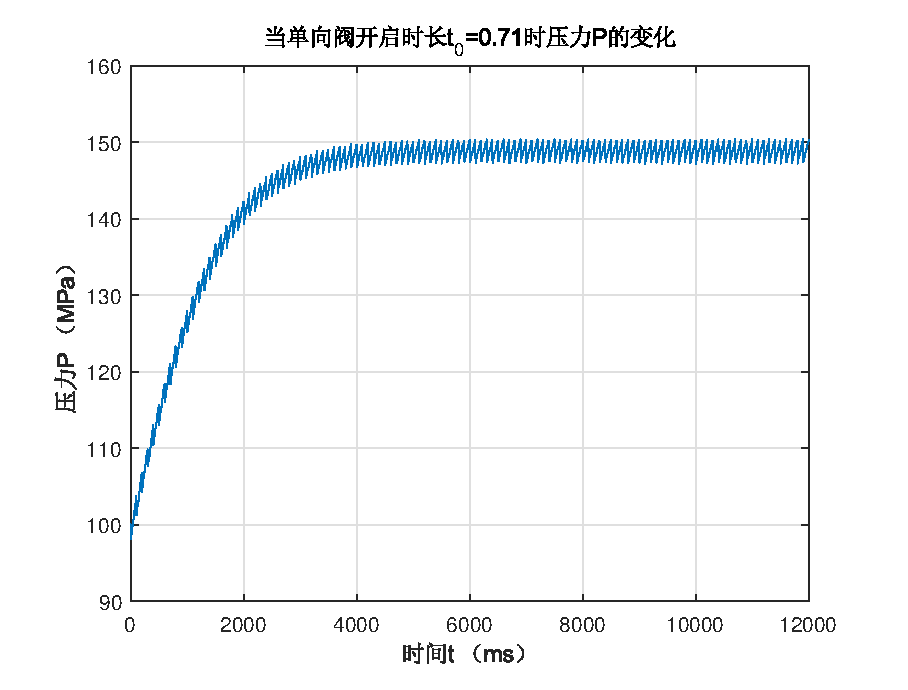
\includegraphics[width=.8\textwidth]{Q1_2runto150in10s}
	\caption{经过10s稳定至150MPa$\,P(t)$图}
	\label{fig:Q1_2runto150in10s}
\end{figure}

\begin{figure}[!h]
	\centering
	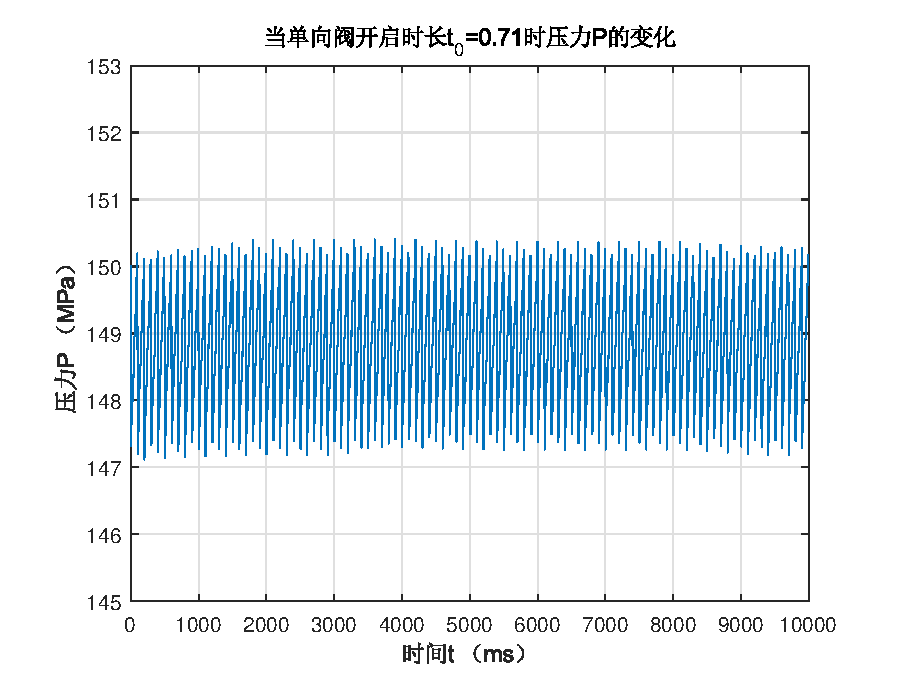
\includegraphics[width=.8\textwidth]{Q1_2keep150}
	\caption{150MPa稳定时$\,P(t)$图}
	\label{fig:Q1_2keep150}
\end{figure}

\subsection{问题二的分析及求解}
\subsubsection{高压油泵供油模型}
由凸轮驱动的高压油泵,其内部的压力不再是某一个常值,而是会根据凸轮的极角的不同而产生不同的压力,如\cref{fig:tulun}所示:



\begin{figure}[!h]
	\centering
	\includegraphics[width=.6\textwidth]{pic3}
	\caption{高压油泵供油示意图}
	\label{fig:tulun}
\end{figure}

当凸轮的极角为$\pi$的时候,柱塞处于下止位点,内部的容积最大,外部的油路会补充柱塞内的燃油,使燃油的压力变为0.5 MPa。当凸轮开始旋转的时候,凸轮推动柱塞向上运动,从而挤压内部的燃油,使得燃油的密度和压力增大,当燃油的压力超过高压油管内部的压力后,单向阀A打开,油泵的液体进入到油管中。柱塞此时仍然会向上运动,直到油泵内的液体的压力无法超过油管内燃油的压力为止。

设凸轮转动的角速度为ω,则凸轮的极角
\begin{equation}
\theta(t)=\omega \cdot t
\end{equation}
由附件一可知,凸轮的极径与凸轮极角的变化角。用$r(\theta)$表示当极角为$\theta$时,凸轮的极径大小。

由以上工作原理易得,高压油泵的容积随极径的变化公式为:
 \begin{equation} \label{eq:Vt-r}
 V(t)=V_0+\pi R^2_b[r(0)-r(\theta)]^2
 \end{equation}
其中,常数项$V_0=20$为极径最大时,高压油泵的残余体积。

将$\theta(t)=\omega \cdot t$、$V_0=20\,\text{mm}^3$、$R_b=2.5\,\text{mm} $、$r(0)=7.239\,\text{mm}$带入式\cref{eq:Vt-r}

得到高压油泵的容积随时间变化的关系式
\begin{equation}
V(t)=20+\pi (2.5)^2\times [7.239-r(\omega \cdot t)]
\end{equation}

为了能够准确判断在某一极短的时间间隔$\Delta t$内油泵内的燃油是否进入了高压油管,我们不妨引入两个中间变量虚燃油密度$\widetilde{\rho}$和虚燃油压力$\widetilde{P}$,用这两个变量表示不发生燃油交换的情况下,经过$\Delta t$时间后的高压油泵内燃油的密度和压力。

在某一时刻$t$,虚燃油参数和实际的燃油参数有如下关系:
%大括号

\begin{equation}
\left\{
\begin{array}{lr}
P(t)\le \widetilde{P}(t), &  \\
\rho(t)\le \widetilde {\rho}(t), &  
\end{array}
\right.
\end{equation}

当且仅当在$\Delta t$内未发生燃油交换的情况下,虚燃油密度$\widetilde{\rho}$等于实燃油密度$\rho$。

设在某一时刻$t-\Delta t$时,高压油泵内的燃油密度为$\rho(t-\Delta t)$,压力为$P(t-\Delta t)$。则经过一极短时间$\Delta t$后,虚燃油密度为$\widetilde{\rho}(t)$。

由
\begin{equation}
\rho(t-\Delta t) \cdot V(t-\Delta t)=\widetilde{\rho}(t) \cdot V(t)
\end{equation}

可得

\begin{equation}
\widetilde{\rho}(t)=\rho(t-\Delta t) \cdot \frac{V(t-\Delta t)}{V(t)}
\end{equation}

若$\widetilde{P}(t) \le P_a(t)$,表示高压油泵内燃油的压力小于等于高压油管内的燃油压力,不会发生燃油交换,实燃油参数等于虚燃油参数。

\begin{equation}
\left\{
\begin{array}{lr}
P(t)=\widetilde{P}(t), &  \\
\rho(t)=\widetilde{\rho}(t), &  
\end{array}
\right.
\end{equation}

若$\widetilde{P}(t)>  P_a(t)$,表示高压油泵内燃油的压力大于高压油管内的燃油压力,泵内的液体会进入到油管内,供油的速率$Q_i(t)$满足如下关系式:

\begin{equation}
A_i=\pi \cdot r^2
\end{equation}
\begin{equation} \label{eq:Qi(t)}
Q_i(t)=C\cdot A_i \sqrt{\frac{2[\widetilde{P}(t)-P_a(t)]}{\widetilde{\rho}(t)}}
\end{equation}

则实际的$\rho(t)$为

\begin{equation}
\rho(t)=\widetilde{\rho}(t)-\frac{Q_i \cdot\widetilde{\rho}(t) \cdot \Delta t}{V(t)}
\end{equation}

综上所述,高压油泵内的液体密度在一个供油周期内随时间变化的函数关系式为:

%对齐

\begin{equation} \label{eq:32}
\widetilde{\rho}(t)=\rho(t-\Delta t) \cdot \frac{V(t-\Delta t)}{V(t)}
\end{equation}




\begin{equation} \label{eq:33}
\rho(t)=\left\{
\begin{array}{lcr}
\widetilde{\rho}(t) & & {\widetilde{P}(t)\le P(t)}\\
\widetilde{\rho}(t)[1-\frac{Q_i(t) \cdot  \Delta t}{V(t)} ]& & {\widetilde{P}(t)>P(t)}
\end{array}
\right.
\end{equation}





\subsubsection{喷油嘴喷油模型}

对于针阀式喷油嘴来说,实际喷孔面积并非是底部最下端的喷油孔,而是针阀升起后针阀下底面与密封座之间的环状空隙,为了叙述方便,用漏环来代指这一环状空隙,$A_o$表示这一环状空隙的面积。如\cref{fig:pic2}所示:
\begin{figure}[!h]
	\centering
	\includegraphics[width=.40\textwidth]{pic2}
	\caption{针阀运动示意图}
	\label{fig:pic2}
\end{figure}

当针阀的升程$x=0$的时候,针阀恰好卡在密封座上,漏环面积$A_o=0$,此时没有燃油从喷油孔喷出;

在一个周期内,我们将针阀的升程$x$与时间$t$之间的离散对应关系记为$x(t)$。取时间间隔$\Delta t=0.01\,$ms,在一个周期内,经过了$n$个$\Delta t$时间后,针阀的升程大小为$x(n\cdot \Delta t)$。

针阀底部中心到密封座的垂线距离$r$与底部中心到顶角的距离$h$满足以下关系式:

\begin{equation}
\frac{r}{h}=\tan 9°
\end{equation}

\begin{equation}
h(x)=h(0)+x
\end{equation}

其中,$h(0)$为生成$x=0$时,下底座中心与圆锥顶角的距离常量。

\begin{equation}
h(0)=\frac{R}{\tan 9°}
\end{equation}

所以

\begin{equation}
r=\tan 9° \cdot(\frac{R}{tan9°}+x)
\end{equation}

由于漏环面积$A_o$的面积计算公式如下:

\begin{equation}
A_B=\pi r^2-\pi R^2
\end{equation}

代入计算得如下公式,其中$R$为针阀的半径。

\begin{equation}
A_{o}(t)=\pi\left[R+\tan 9° \cdot x(t)\right]^2-\pi R^2
\end{equation}

那么在某一时刻$t$时,喷油嘴的喷油速率为:
\begin{equation}
Q_{o}(t)=C\cdot A_{o} \sqrt{\frac{2\left(P(t)-P_{r}\right)}{\rho_{a}(t)}}
\end{equation}

其中$P_{r}=12.0\,\text{MPa}$\upcite{bib:5},表示发动机燃烧室的压力。

\subsubsection{高压油管内的燃油压力和密度变化模型}

联立\cref{eq:rho_{a}(t)} \cref{eq:P_{a}(t)} \cref{eq:Qi(t)} \cref{eq:32} \cref{eq:33}式可得:

\begin{equation}
\rho_a(t)=\rho_a(t-\Delta t)+\frac{Q_i(t) \widetilde{\rho}(t)-Q_{o}(t)\rho_{a}(t-dt)}{V_{a}}\Delta t		
\end{equation}

\begin{equation}
P_{a}(t)=\frac{1}{-0.0039} \ln\left[\left(-5.8312 \right)\ln \frac{\rho_a(t)}{0.85}+0.677\right]	
\end{equation}

在$t=0$时,$\rho_a (t)=0.85\,\text{mg/mm}^{3},P_a(t)=100\,\text{MPa}$


在已知初始条件的情况下,我们选取足够小的时间间隔$\Delta t$,然后利用微分方程进行仿真实验,模拟递推出每一时刻油管内部燃油的密度和压力的变化趋势和参数。得到任一时刻油管内部的燃油参数。
\subsubsection{问题二的求解结果}

我们取$\Delta t=$0.01 ms,利用变步长搜索搜索法对凸轮旋转角速度$\omega$进行遍历,求出在每一个给定的角速度$\omega_{0}$时,各个时刻的油管燃料压力$P(t)$。利用式\cref{eq:F(omega)}计算出各个角速度所对应的$F(\omega)$,并取使$F(\omega)$取得最小值时的$\omega$为最优角速度,解得$\omega=14.15\pi \, \text{rad/s}$,此时$P(t)$变化如\cref{fig:Q2}所示:


\begin{equation} \label{eq:F(omega)}
 F(\omega)=\sum_{n=0}^N[P_{a}(n\Delta t)-P_{a}(0)]^2
\end{equation}

\begin{figure}[!h]
	\centering
	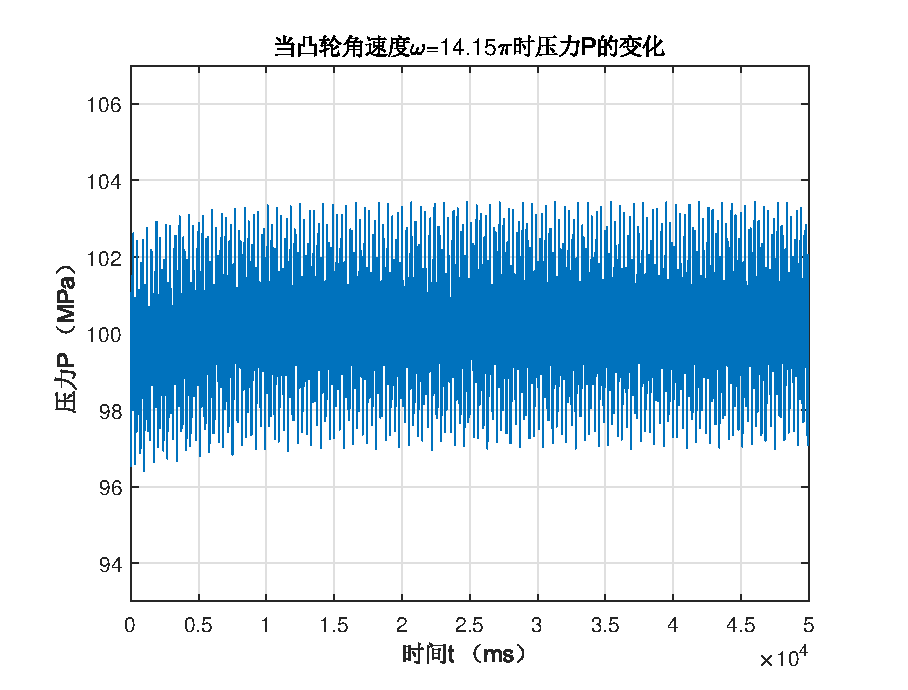
\includegraphics[width=.8\textwidth]{Q2}
	\caption{$\omega=14.15\pi$时压力$P$变化图}
	\label{fig:Q2}
\end{figure}

\subsection{问题三的分析及求解}

\subsubsection{引入新喷油嘴C后的高压油管燃油压力和密度变化模型}

新引入喷油嘴C与喷油嘴B的针阀运动规律相同且在开启时都为$x(t)$(详见附件三)。

若喷油嘴B和喷油嘴C在一个供油周期总是同步工作的,则必然会导致高压油管的压力变化速度过快,不利于高压油管保持稳定。所以,我们在两个喷油嘴每秒工作十次的基础上,寻找到最佳的各自开启时间。

在100 ms的喷油嘴工作周期内,设喷油嘴B的开启时间为$t_{B}$、喷油嘴C的开启时间为$t_{C}$,则两喷油嘴的针阀运动规律如下:

\begin{equation}
x_{B}(t)=\left\{
\begin{array}{lcr}
x(t-t_{B}) & & {t \in [t_{B},t_{B}+2.45]}\\
0 & &{\text{其他}}
\end{array} \right.
\end{equation}

\begin{equation}
x_{C}(t)=\left\{
\begin{array}{lcr}
x(t-t_{C}) & & {t \in [t_{C},t_{C}+2.45]}\\
0 & &{\text{其他}}
\end{array} \right.
\end{equation}

所以两喷油嘴的喷油速率。

\begin{equation}
Q_{OB}(t)=C \cdot A_{OB}(t) \sqrt{\frac{2 \cdot (P_{a}(t)-P_{C})}{\rho_{a}(t)}}
\end{equation}

\begin{equation}
Q_{OC}(t)=C \cdot A_{OC}(t) \sqrt{\frac{2 \cdot (P_{a}(t)-P_{C})}{\rho_{a}(t)}}
\end{equation}

\begin{equation}
Q_{O}(t)=C \cdot A_{OB}(t) \sqrt{\frac{2 \cdot (P_{a}(t)-P_{C})}{\rho_{a}(t)}}+C \cdot A_{OC}(t) \sqrt{\frac{2 \cdot (P_{a}(t)-P_{C})}{\rho_{a}(t)}}
\end{equation}

所以,对于有两个喷油嘴的高压油管燃油的压力和密度变化模型,只需将原模型\cref{eq:rho_{a}(t)}中的$Q_{O}(t)$作如上修正即可。






\subsubsection{建立优化目标评价体系}

\textbf{优化目标一:减小最大压力差}

根据我们的初步计算,无论如何给定凸轮角速度$\omega$、两喷油嘴开启时间$t_{B}$和$t_{C}$,经过一段时间后,燃油压力总会围绕某一固定值上下震荡。计$G(\omega,t_{B},t_{C})$为给定如上条件下高压油管的压力与标准100MPa之间的最大压力差。

即
\begin{equation}
G(\omega,t_{B},t_{C})=max{(P_{a}(t)-P_{a}(0))} 
\end{equation}

其中$P_{a}(0)$表示标准燃油压力100MPa。

在问题二中,我们计算出的凸轮角速度$w=14.15\pi\, \text{rad/s}$的情况下,最大压力差为$G_{0}=7.031\,\text{MPa}$。那么在问题三中,既然有两个喷油嘴可供我们调配,则问题三的最大压力差$G(\omega,t_{B},t_{C})$应小于或等于问题二中的最大压力差$G_{0}$。

即
\begin{equation}
G(\omega,t_{B},t_{C}) \le G_{0}
\end{equation}

\textbf{优化目标二:压力差平方和最小}

每给定一组$(\omega,\,t_{B},\,t_{C})$,我们就可以通过公式计算得出一段时间内的平方和,则使得平方和最小的一组解,即为使得系统保持稳定的最优解。

\begin{equation} 
F=\sum_{n=0}^{N}[P_a(n\Delta t)-P_a(0)]^2
\end{equation}


\subsubsection{控制变量法研究组件的工作特性}

对于研究新增添减压阀后的高压油管的供油和喷油策略,我们不妨首先利用控制变量法,研究减压阀和喷油嘴各自的工作特性,并根据他们具体的工作特性来制定最优的供油和喷油策略。

先将减压阀从系统中排除,考虑一个喷油嘴对高压油管压力的影响。
\clearpage

固定喷油嘴的开启时间为$t=0$时刻,取$\Delta \omega=2\,\text{rad/s}$,利用MATLAB软件分别画出在每一个供油周期内,角速度从$10\,\text{rad/s}$到$20\,\text{rad/s}$的一簇变化曲线,如\cref{fig:omegabh10-20}所示:

\begin{figure}[!h]
	\centering
	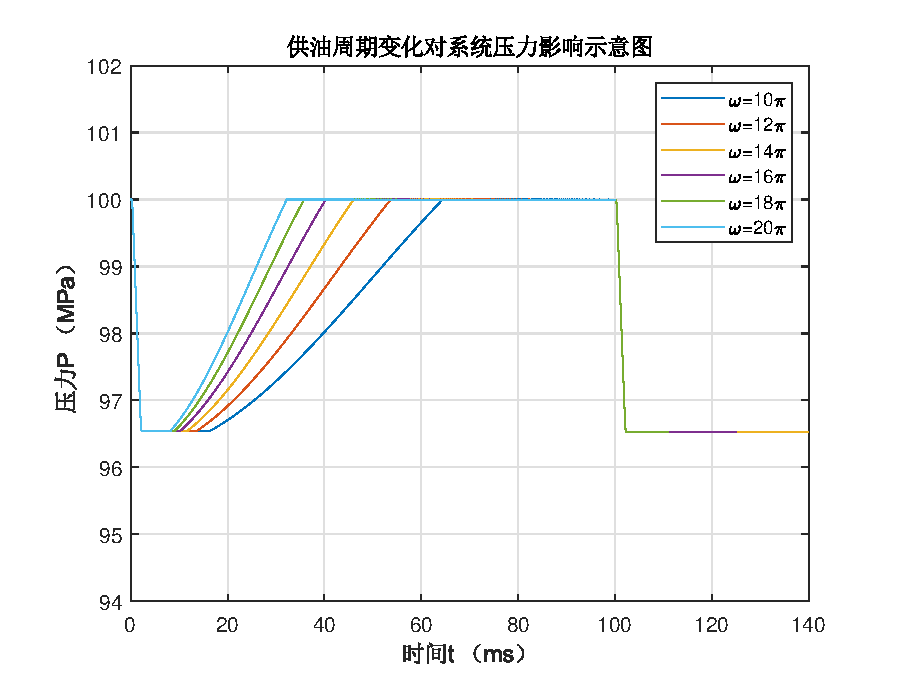
\includegraphics[width=.7\textwidth]{omegabh10-20}
	\caption{供油周期变化对系统压力影响示意图}
	\label{fig:omegabh10-20}
\end{figure}


固定凸轮角速度$\omega =15\,\text{rad/s}$,取$\Delta t=10\,\text{ms}$,利用MATLAB软件分别画出在每一个供油周期内,开启时间从$45\, \text{ms}$到$65 \, \text{ms}$的一簇变化曲线,如\cref{fig:pyzbh45-65}所示:


\begin{figure}[!h]
	\centering
	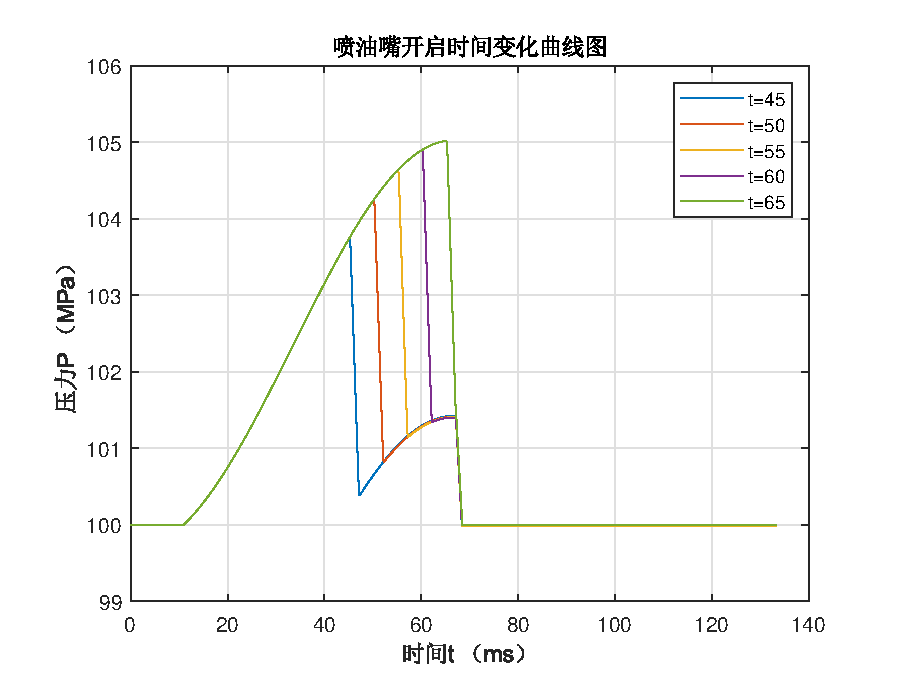
\includegraphics[width=.7\textwidth]{pyzbh45-65}
	\caption{喷油嘴开始时间变化对系统压力影响示意图}
	\label{fig:pyzbh45-65}
\end{figure}


通过比较图 和图 可以发现,当系统中只存在喷油嘴时,系统的压力会先增大后减小再增大,并最终停留在压力高于100 MPa的某个稳态上。

将喷油嘴从系统中排除,单考虑减压阀对高压油管压力的影响。

取$\Delta P=1\,\text{MPa}$,利用MATLAB软件画出用减压阀将系统的原稳态压力下降到100MPa的一簇变化曲线,原系统的的稳态压力从101 MPa到105 MPa不等,如\cref{fig:jyfbh101-105}所示:


\begin{figure}[!h]
	\centering
	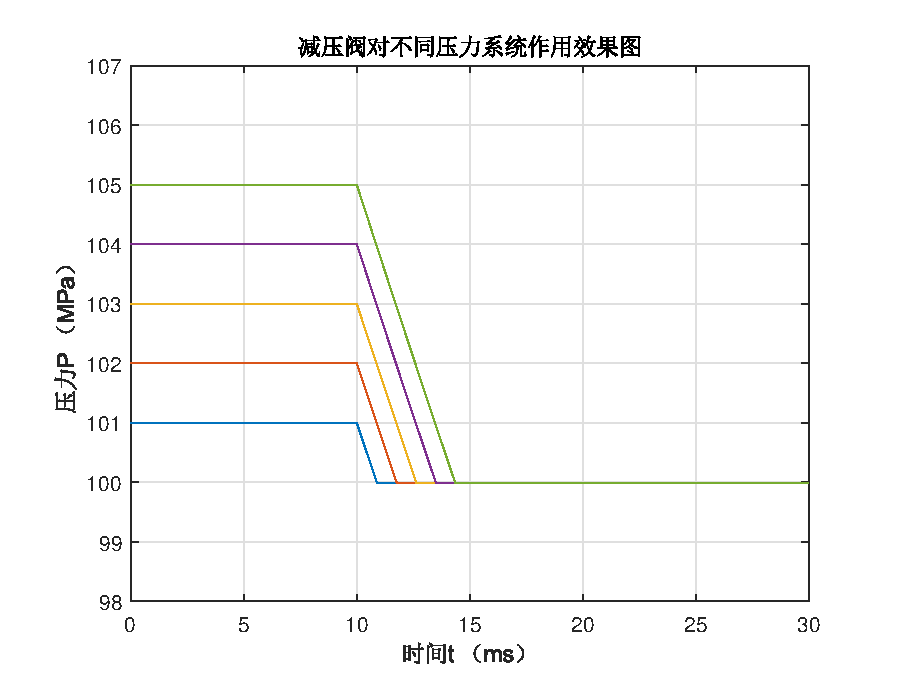
\includegraphics[width=.8\textwidth]{jyfbh101-105}
	\caption{喷油嘴开始时间变化对系统压力影响示意图}
	\label{fig:jyfbh101-105}
\end{figure}


分析以上各图,我们可以发现:利用减压阀,可以精确地在一个较短的时间内把系统的压力下降到100 MPa。利用MATLAB软件计算可以得出,利用减压阀将系统压力从101.5 MPa到100 MPa的下降时间$t^{'}\approx 1.30\,\text{ms}$,远小于$\omega=15\,\text{rad/s}$时的系统供油周期$T=418.9\,\text{ms}$。
即
\begin{equation}
t^{'}\ll  T
\end{equation}
所以,根据减压阀和喷油嘴调控系统压力的特点,我们制定如下策略:

设凸轮转动的角速度为ω,则供油周期$T=\frac{2 \pi}{ \omega}$

当$t=0$时,系统的$P_{a}(t)=0$减压阀和喷油嘴都处于关闭状态,此时凸轮刚开始旋转。

当$t=t_{p}$时,高压油泵的压力达到临界状态,高压油泵开始向油管里供油。

当$t=t_{0}$时,单个喷油嘴B开始工作,高压油管开始向外界喷射油滴。

当$t=t_{0}+2.45$时,喷油嘴工作结束,系统不再通过喷油嘴向外界喷油,但高压油管继续向系统供油。 

当$t=t_{s}$时,高压油泵达到下临界状态,无法再向系统内供油。

当$t=t_{k}$时,减压阀开始工作,系统的压力开始下降。

当$t=t_{d}$时,系统的压力回到100 MPa,减压阀关闭,直到下一个周期循环开始。

当$t=T$时,一个完整的供油周期结束,$P$和$\rho$回到t=0时的状态。

控制方案如\cref{fig:kzfa}所示:

\begin{figure}[!h]
	\centering
	\includegraphics[width=.8\textwidth]{kzfa}
	\caption{油泵与减压阀控制方案示意图}
	\label{fig:kzfa}
\end{figure}



\subsubsection{问题三求解}

对于第一问,我们取$\Delta t=0.01\,\text{ms}$,利用变步长搜索法对凸轮角速度$ω$、喷油嘴B的开启时间$t_{B}$、喷油嘴C的开启时间$t_{C}$。在依次满足第一优化目标和第二优化目标的情况下,计算得到最优的供油和喷油系统设计方案为:凸轮角速度$\omega=28.34\pi\,$rad/s,喷油嘴B开启时间为1.1 ms、喷油嘴C的开启时间为50.4 ms,此时系统的稳定性最佳。



在此设计方案下,系统的压力$P$随时间变化的曲线图如\cref{fig:Q3_1r}所示:

\clearpage

\begin{figure}[!h]
	\centering
	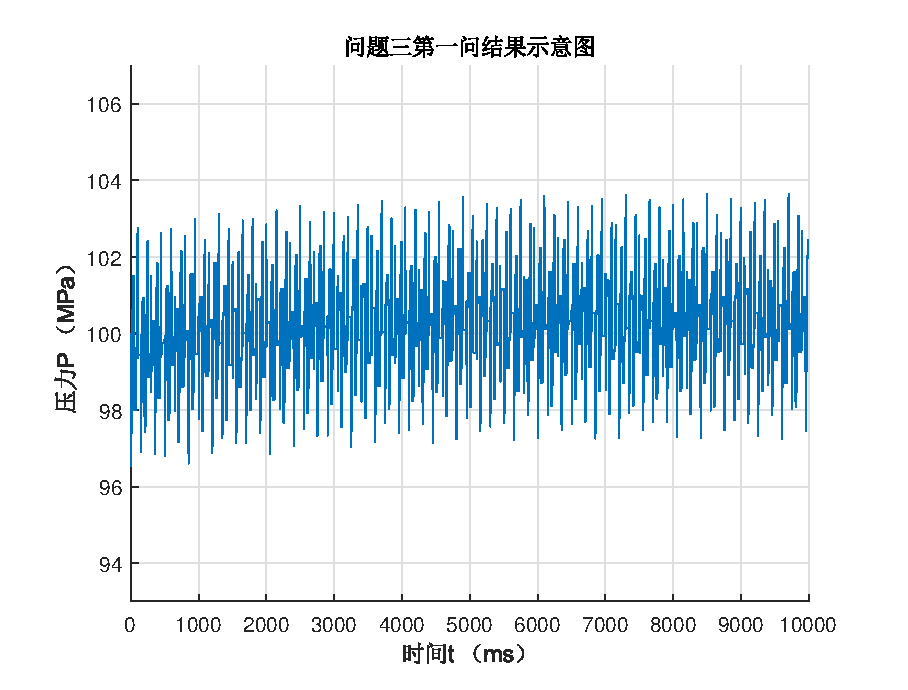
\includegraphics[width=.8\textwidth]{Q3_1r}
	\caption{问题三第一问结果示意图}
	\label{fig:Q3_1r}
\end{figure}


对于第二问,我们初步计算后发现,在满足第一优化目标$G(\omega,t_{B},t_{C}) \le G_{0}$的情况下,一定范围内,第二优化目标$F(\omega)$随着$\omega$的变大而减小。考虑到一般柴油发动机柱塞凸轮的转动速度最大不超过$1600\,\text{r/min}$,即$\omega=53.33\,\text{rad/s}$便为最优角速度,在这个条件下,通过最优目标规划法,给出我们的喷油嘴和减压阀控制方案。



当$t=0$时,系统的$P_{a}(t)=0$,减压阀和喷油嘴都处于关闭状态,此时凸轮刚开始旋转。

当$t=3.09\,\text{ms}$时,高压油泵的压力达到临界状态,高压油泵开始向油管里供油。

当$t=6.86\,\text{ms}$时, 单个喷油嘴B开始工作,高压油管开始向外界喷射油滴。

当$t=9.34\,\text{ms}$时,喷油嘴工作结束,系统不再通过喷油嘴向外界喷油,但高压油管继续向系统供油。 

当$t=18.74\,\text{ms}$时,高压油泵达到下临界状态,无法再向系统内供油。

当$t=18.89\,\text{ms}$时,减压阀开始工作,系统的压力开始下降。 

当$t=20.19\,\text{ms}$时,系统的压力回到100MPa,减压阀关闭,直到下一个周期循环开始。

当$t=37.51\,\text{ms}$时,一个完整的供油周期结束,$P$和$\rho$回到t=0时的状态。

控制方案如\cref{fig:Q32o}所示:


\begin{figure}[!h]
	\centering
	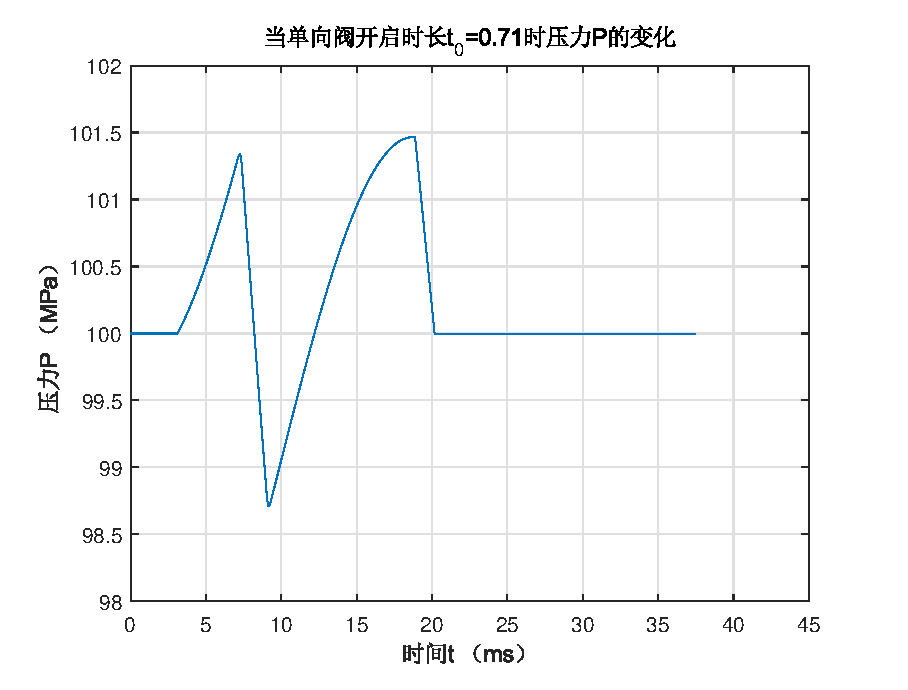
\includegraphics[width=.8\textwidth]{Q32o}
	\caption{油泵与减压阀控制方案示意图}
	\label{fig:Q32o}
\end{figure}










\section{模型的应用及推广}


单体泵是现代汽车工业实现清洁燃烧的一项重要的技术,由柱塞泵、高压油管以及喷油器构成。我们以本世纪初曾大量投入生产的柴油发动机的的单体泵系统为例,考虑本模型在实际高压油管单体泵系统上的应用\upcite{bib:6}。

提取本类型柴油机的相关参数,柱塞腔内半径为7.5 mm,柱塞运动到下止位点时,柱塞腔长度为34.8 mm,低压燃油的压力为10.0 MPa;柱塞运动到上止位点时,升程为19mm。驱动柱塞运动的曲轴的转速为1250 r/min。高压油管的长度为320 mm,半径为1.5 mm,工作时,压力稳定在170 MPa左右。以上工作原理和参数符合我们所建立的高压油管内燃油压力和密度变化模型,我们将相关数据带入,来检验我们的模型。

我们将数据代入模型中进行计算,发现在$\rho=0.95\,\text{mg/mm}^{3}$之前,模型与实际符合良好。但当油泵内液体的密度达到$0.95\,\text{mg/mm}^{3}$之后,根据微分方程所求出的数据结果与实际情况差别过大,利用MATLAB进行大规模数值求解后发现,此时微分方程仅仅存在复数解。

对结果进行分析后可以发现,我们建立的密闭容器内燃油压力$P$与密度ρ的公式存在适用范围。只有燃油密度$\rho < 0.95\,\text{mg/mm}^{3}$或燃油压力$P< 912.45\,\text{MPa} $的燃油,才可以带入公式进行计算。$\rho=0.95 \,\text{mg/mm}^{3}$ 便为此模型下的极限压缩密度,在燃油密度达到这个极限点后便无法再继续压缩。查阅相关文献\upcite{bib:7}可以得知,实际燃油的极限压缩密度只能达到$0.90\,\text{mg/mm}^{3}$。而我们的模型并没有充分考虑到这一点,使得燃油密度公式在高密度部分存在一定量的误差。如若能根据液体的这一特性对公式进行修正,则得到的模型更佳。

\section{模型的优缺点}
\subsection{模型的优点}



\begin{enumerate}
	\item 考虑了发动机中高压油管的实际工作情况,在明确发动机中高压油管工作原理的情况下,研究高压油管各组件的功能与用途,在此基础上,最大程度的还原了高压油管各组件的实际工作规律与模式。
	\item 采用多目标优化法建立模型,综合考虑高压油管各方面的功能和效用,利用此方法解得的模型结果的可信度高,模型结果更符合题目要求。
	\item 模型采用仿真模拟算法,计算结果与实际情况契合程度高。
	\item 将所建模型应用于实际柴油发动机,与实际高压油管参数做对比,可对模型的实用性进行评估。
\end{enumerate}

\subsection{模型的缺点}



\begin{enumerate}

\item 模型具有一定的局限性。只适用于高压油管内液体密度为$\rho<0.95\,\text{mg/mm}^{3}$的情况,当高压油管内液体密度超出范围时,模型不再适用。
\end{enumerate}

\newpage

%参考文献
\begin{thebibliography}{9}%宽度9
	
	\bibitem[1]{bib:1}姜峰, 梁霖, 莫清烈, 罗建斌, 郝真真. 电控单体泵燃用生物柴油嘴端压力波动仿真分析[J]. 广西科技大学学报, 2018, 29(01):81-85+105.
	\bibitem[2]{bib:2}韩江枫, 王祥, 尹长城. 基于有限元法发动机高压油管的模态分析[J]. 湖北汽车工业学院学报, 2018, 32(04):11-13+21.
	\bibitem[3]{bib:3}Mathematical model of diesel fuel injection equipment incorporating non-linear fuel injection. Lee, H.-K.,Russell, M.F.,Bae, C.S. Proceedings of the Institution of Mechanical Engineers, Part D: Journal of Automobile Engineering . 2002
	\bibitem[4]{bib:4}苏海峰, 李鹏志, 郝刚, et al. 喷油脉宽对高压共轨多次喷射油量波动的影响规律[J]. 车用发动机, 2011(6):38-41.
	\bibitem[5]{bib:5}韦学元. 发动机燃烧室内部压力测量技术[J]. 计量技术, 2017:32.
	\bibitem[6]{bib:6}张海磊, 王强, 冯耀楠. 高压油管长度对柱塞泵结构强度的影响[J]. 机床与液压, 2019, 47(08):103-108.
	\bibitem[7]{bib:7}天津大学, 山西潞安矿业(集团)有限责任公司. 一种高密度柴油及其制备方法:CN201610888293. 0[P]. 2017-01-18.
\end{thebibliography}

\newpage
%附录
\begin{appendices}


\section{问题1-稳定100MPa}

\begin{lstlisting}[language=matlab]
% 2019_A
% time: 2019/09/12 21:50

% Task: keep 100MPa
clear all;
Rho_fuel = 0.850; % unit mg/mm^3
C= 0.85 ; %Flow Coefficient
A= pi*0.7^2; % Area of the small hole. unit is mm^2

V_tube=pi*500*5^2;
Rho_160 = exp(-(1/(0.0039*exp(7.31)))*(exp(-0.0039*160)-exp(-0.39)) + log(0.85))  ; % Fuel density at a pressure of 160 MPa
i=1;
data=zeros(10000,1);
for T=0.289 % unit is ms. The time each time the one-way valve is opened
    a=0;
    b=0.01;
    c=100000;
    n=(c-a)/b + 1;
    P_aims=100;
    Rho_fuel_i=zeros(n,1);
    P_tube_i=zeros(n,1);
    k=1;
    Rho_fuel_i(k,1)=Rho_fuel;
    for t=a:b:c % unit is ms. Simulate the entire working time frame
        
        P_tube_i(k,1) = log(-(log(Rho_fuel_i(k,1)/Rho_fuel) - (exp(-0.39)/(0.0039*exp(7.31))))*0.0039*exp(7.31))*(-1/0.0039);
        
        t_fuel_in=mod(t,T+10); % Fuel s cycle time
        t_fuel_out=mod(t,100); % Fuel injection cycle time
        if t_fuel_in>0 && t_fuel_in<=T && P_tube_i(k,1) <=160
           Q_in = C*A*sqrt(2*(160-P_tube_i(k,1))/Rho_160)*b;
        else
            Q_in=0;
        end

        if 0<t_fuel_out && t_fuel_out < 0.2 
           Q_out = 100*t_fuel_out * b;
        elseif 0.2 <= t_fuel_out && t_fuel_out<2.2
           Q_out = 20 * b;
        elseif 2.2 <= t_fuel_out && t_fuel_out<=2.4
           Q_out = (-100*t_fuel_out+240) * b;
        else
           Q_out = 0;
        end
        
        Rho_fuel_i(k+1,1) = (Rho_fuel_i(k,1) * (V_tube- Q_out) + Rho_160 * Q_in) /V_tube;
        
        k=k+1;
    end
    variance=sum((P_tube_i-P_aims).^2);
    data(i,1)=T;
    data(i,2)=variance;
    plot(a:b:c,P_tube_i);
    i=i+1;
end

\end{lstlisting}
\section{问题1-指定时间增长至150MPa} 
\begin{lstlisting}[language=matlab]
% 2019_A Q1_(2) run to 150
% time: 2019/09/13 10:36

% Task: Increase to 150MPa in n seconds
clear all;
Rho_fuel = 0.850; % unit mg/mm^3
P_A = 160; % unit is MPa
P_tube=100; % unit is MPa. Pressure of high pressure oil pipe in initial state
C= 0.85 ; %Flow Coefficient
A= pi*0.7^2; % Area of the small hole. unit is mm^2

V_tube=pi*500*5^2;
Rho_160 = exp(-(1/(0.0039*exp(7.31)))*(exp(-0.0039*160)-exp(-0.39)) + log(0.85)) ; % Fuel density at a pressure of 160 MPa
i=1;
for T=0.71 % unit is ms. The time each time the one-way valve is opened1
    a=0;
    b=0.01;
    c=12*1000;% Adjust the time
    n=(c-a)/b + 1;
    P_aims=150; % new aims
    %Rho_fuel_i=zeros(n+1,1);
    %P_tube_i=zeros(n+1,1);
    k=1;
    Rho_fuel_i(k,1)=Rho_fuel;
    for t=a:b:c % unit is ms. Simulate the entire working time frame
        if k==1
           P_tube_i(1,1)=100;
        else
           P_tube_i(k,1) = log(-(log(Rho_fuel_i(k,1)/Rho_fuel) - (exp(-0.39)/(0.0039*exp(7.31))))*0.0039*exp(7.31))*(-1/0.0039);
        end
        t_fuel_in=mod(t,T+10); % Fuel s cycle time
        t_fuel_out=mod(t,100); % Fuel injection cycle time
        if t_fuel_in>0 && t_fuel_in<=T && P_tube_i(k,1) <=160
           Q_in = C*A*sqrt(2*(160-P_tube_i(k,1))/Rho_160)*b;
        else
            Q_in=0;
        end

        if 0<t_fuel_out && t_fuel_out < 0.2 
           Q_out = 100*t_fuel_out * b;
        elseif 0.2 <= t_fuel_out && t_fuel_out<2.2
           Q_out = 20 * b;
        elseif 2.2 <= t_fuel_out && t_fuel_out<=2.4
           Q_out = (-100*t_fuel_out+240) * b;
        else
           Q_out = 0;
        end
        
        Rho_fuel_i(k+1,1) = (Rho_fuel_i(k,1) * (V_tube- Q_out) + Rho_160 * Q_in) /V_tube;
        
        k=k+1;
    end
    variance=(P_tube_i(n)-P_aims)^2;
    data(i,1)=T;
    data(i,2)=variance;
    i=i+1;
end

\end{lstlisting}

\section{问题1-稳定150MPa} 
\begin{lstlisting}[language=matlab]
% 2019_A Q1_(2)
% time: 2019/09/13 10:20

% Task: keep 150MPa

clear all;
Rho_fuel = 0.850; % unit mg/mm^3
P_A = 160; % unit is MPa
P_tube=100; % unit is MPa. Pressure of high pressure oil pipe in initial state
C= 0.85 ; %Flow Coefficient
A= pi*0.7^2; % Area of the small hole. unit is mm^2

V_tube=pi*500*5^2;
Rho_160 =exp(-(1/(0.0039*exp(7.31)))*(exp(-0.0039*160)-exp(-0.39)) + log(0.85)); % Fuel density at a pressure of 160 MPa
Rho_150 = exp(-(1/(0.0039*exp(7.31)))*(exp(-0.0039*150)-exp(-0.39)) + log(0.85));
i=1;
for T=0.71 % unit is ms. The time each time the one-way valve is opened
    a=0;
    b=0.01;
    c=200000;
    n=(c-a)/b + 1;
    P_aims=150*ones(n,1);
    %Rho_fuel_i=zeros(n+1,1);
    %P_tube_i=zeros(n+1,1);
    k=1;
    Rho_fuel_i(k,1)=Rho_150;
    for t=a:b:c % unit is ms. Simulate the entire working time frame
        if k==1
            P_tube_i(1,1)=150;
        else
            P_tube_i(k,1) = log(-(log(Rho_fuel_i(k,1)/Rho_fuel)-((exp(-0.39))/(0.0039*exp(7.31))))*0.0039*exp(7.31))*(-1/0.0039);
        end
        
        t_fuel_in=mod(t,T+10); % Fuel s cycle time
        t_fuel_out=mod(t,100); % Fuel injection cycle time
        if t_fuel_in>0 && t_fuel_in<=T && P_tube_i(k,1) <=160
            Q_in = C*A*sqrt(2*(160-P_tube_i(k,1))/Rho_160)*b;
        else
            Q_in=0;
        end

        if 0<t_fuel_out && t_fuel_out < 0.2 
           Q_out = 100*t_fuel_out * b;
        elseif 0.2 <= t_fuel_out && t_fuel_out<2.2
           Q_out = 20 * b;
        elseif 2.2 <= t_fuel_out && t_fuel_out<=2.4
           Q_out = (-100*t_fuel_out+240) * b;
        else
           Q_out = 0;
        end
        
        Rho_fuel_i(k+1,1) = (Rho_fuel_i(k,1) * (V_tube- Q_out) + Rho_160 * Q_in) /V_tube;
        
        k=k+1;
    end
    variance=sum((P_tube_i-P_aims).^2);
    data(i,1)=T;
    data(i,2)=variance;
    i=i+1;
	plot(a:b:c,P_tube_i)
    ylim([90,160]);
end

\end{lstlisting}


\section{问题2求解} 
\begin{lstlisting}[language=matlab]
% 2019_A Q2
% time: 2019/09/13 13:23

clear all;
Rho_fuel = 0.850; % unit mg/mm^3
C= 0.85 ; %Flow Coefficient
A_in= pi*0.7^2; % Area of the small hole. unit is mm^2


% Needle valve motion data
load('Needle.mat');
% Cam edge data
load('Cam.mat');

V_tube=pi*500*5^2;
Rho_160 = exp(-(1/(0.0039*exp(7.31)))*(exp(-0.0039*160)-exp(-0.39)) + log(0.85)); % Fuel density at a pressure of 160 MPa
Rho_0_5= exp(-(1/(0.0039*exp(7.31)))*(exp(-0.0039*0.5)-exp(-0.39)) + log(0.85)); % Fuel density at a pressure of 0.5 MPa
i=1;
data=zeors(10000,1);
for omega=14.15*pi % unit is rad/s . Cam angular velocity
    clear Rho_fuel_i P_tube_i theta V_pump h_Needle Rho_pump_i P_pump_i m_Q_in A_out m_Q_out
    a=0;
    b=0.01;
    c=100000;
    n=(c-a)/b + 1;
    P_aims=100;
    
    % Allocate memory
    Rho_fuel_i=zeros(n,1);
    P_tube_i=zeros(n,1);
    theta=zeros(n,1);
    V_pump=zeros(n,1);
    h_Needle=zeros(n,1);
    Rho_pump_i=zeros(n,1);
    P_pump_i=zeros(n,1);
    m_Q_in=zeros(n,1);
    A_out=zeros(n,1);
    m_Q_out=zeros(n,1);
    
    k=1;
    Rho_fuel_i(k,1)=Rho_fuel;
    P_tube_i(k,1)= 100;
    for t=a:b:c % unit is ms. Simulate the entire working time frame
        theta(k,1)=mod(pi+omega*t/1000,2*pi); % The polar angle of the current moment cam. (unit is rad)
        n_R= floor(theta(k,1)*100); % Theta index in Cam data
        R_theta = (Cam(mod(n_R+1,628)+1,2)-Cam(mod(n_R,628)+1,2))*(theta(k,1)*100-n_R)+Cam(mod(n_R,628)+1,2) ; % The diameter of the current moment cam. (unit is mm)
        V_pump(k,1) = 20+pi*(5/2)^2*(Cam(1,2)-R_theta); % Relationship between oil pump volume and pole diameter.
        
        Needle_t=floor(mod(100*t,100*100)+1); %Index of time t in Needle data
        if Needle_t<247
            h_Needle(k,1)=Needle(Needle_t,2); % h is the Lift of Needle.
        else
            h_Needle(k,1)=0;
        end
        if k==1
            Rho_pump_i(k,1)= Rho_0_5; 
        else
            if floor(mod(100*t,100*1000*(2*pi)/omega))==0
                Rho_pump_i(k,1)= Rho_0_5;
            else
                Rho_pump_i(k,1)=Rho_pump_i(k-1,1)*V_pump(k-1,1)/V_pump(k,1); % Fuel density in the oil pump at the current time.
            end
        end
        P_pump_i(k,1) = log(-(log(Rho_pump_i(k,1)/Rho_fuel) - (exp(-0.39)/(0.0039*exp(7.31))))*0.0039*exp(7.31))*(-1/0.0039);
        if k>1 
            if Rho_pump_i(k,1)>Rho_fuel_i(k-1,1) 
                m_Q_in(k,1)=C*A_in*sqrt(2*(P_pump_i(k,1) - P_tube_i(k-1,1))*Rho_pump_i(k,1))*b;
                Rho_pump_i(k,1)=(Rho_pump_i(k,1)*V_pump(k,1)-m_Q_in(k,1))/V_pump(k,1);
                P_pump_i(k,1) = log(-(log(Rho_pump_i(k,1)/Rho_fuel) - (exp(-0.39)/(0.0039*exp(7.31))))*0.0039*exp(7.31))*(-1/0.0039);
            else
                m_Q_in(k,1)=0;
            end
            A_out(k,1) = pi*((h_Needle(k,1)+1.25/(tan(pi*9/180)))*tan(pi*9/180))^2-pi*1.25^2;
            if P_tube_i(k-1,1)>12 
                m_Q_out(k,1) = C*A_out(k,1)*sqrt(2*(P_tube_i(k-1,1) - 12)*Rho_fuel_i(k-1,1))*b;
            else
                m_Q_out(k,1) = 0;
            end
            Rho_fuel_i(k,1)=(Rho_fuel_i(k-1,1)*V_tube-m_Q_out(k,1)+m_Q_in(k,1))/V_tube;
            P_tube_i(k,1) = log(-(log(Rho_fuel_i(k,1)/Rho_fuel) - (exp(-0.39)/(0.0039*exp(7.31))))*0.0039*exp(7.31))*(-1/0.0039);
        end
        k=k+1;
    end
    variance=sum((P_tube_i-P_aims).^2);
    data(i,1)=omega/pi;
    data(i,2)=variance;
    i=i+1;
    hold on
    plot(a:b:c,P_tube_i)
    % ylim([0,200]);
end

\end{lstlisting}

\section{问题3第一问求解} 
\begin{lstlisting}[language=matlab]

% 2019_A Q3_1_4th
% time: 2019/09/14 14:41

clear all;
Rho_fuel = 0.850; % unit mg/mm^3
P_A = 160; % unit is MPa
P_tube=100; % unit is MPa. Pressure of high pressure oil pipe in initial state
C= 0.85 ; %Flow Coefficient
A_in= pi*0.7^2; % Area of the small hole. unit is mm^2


% Needle valve motion data
load('Needle.mat');
% Cam edge data
load('Cam.mat');

V_tube=pi*500*5^2;
Rho_160 = exp(-(1/(0.0039*exp(7.31)))*(exp(-0.0039*160)-exp(-0.39)) + log(0.85)); % Fuel density at a pressure of 160 MPa
Rho_0_5= exp(-(1/(0.0039*exp(7.31)))*(exp(-0.0039*0.5)-exp(-0.39)) + log(0.85)); % Fuel density at a pressure of 0.5 MPa
i=1;
sign_break = 0;
data=zeros(10000,1);
for omega=6*pi % unit is rad/s . Cam angular velocity
    clear Rho_fuel_i P_tube_i theta V_pump h_Needle1 h_Needle2 Rho_pump_i P_pump_i m_Q_in A_out1 A_out2 m_Q_out
    a=0;
    b=0.01;
    c=10000;
    n=(c-a)/b + 1;
    P_aims=100;
    sign_break = 0;
    
    % Allocate memory
    Rho_fuel_i=zeros(n,1);
    P_tube_i=zeros(n,1);
    theta=zeros(n,1);
    V_pump=zeros(n,1);
    h_Needle1=zeros(n,1);
    h_Needle2=zeros(n,1);
    Rho_pump_i=zeros(n,1);
    P_pump_i=zeros(n,1);
    m_Q_in=zeros(n,1);
    A_out1=zeros(n,1);
    A_out2=zeros(n,1);
    m_Q_out=zeros(n,1);
    
    
    for t1=6 % Range: 0~100, indicating the starting working time of the injector during the period T=100ms.
        for t2=30:50 % Range: 0~100, indicating the starting working time of the injector during the period T=100ms.
            k=1;
            Rho_fuel_i(k,1)=Rho_fuel;
            P_tube_i(k,1)= 100;
            for t=a:b:c % unit is ms. Simulate the entire working time frame
                theta(k,1)=mod(pi+omega*t/1000,2*pi); % The polar angle of the current moment cam. (unit is rad)
                n_R= floor(theta(k,1)*100); % Theta index in Cam data
                R_theta = (Cam(mod(n_R+1,628)+1,2)-Cam(mod(n_R,628)+1,2))*(theta(k,1)*100-n_R)+Cam(mod(n_R,628)+1,2) ; % The diameter of the current moment cam. (unit is mm)
                V_pump(k,1) = 20+pi*(5/2)^2*(Cam(1,2)-R_theta); % Relationship between oil pump volume and pole diameter.

                % Fuel injector 1
                Needle_t1=floor(mod(100*((100-t1)+t),100*100)+1); %Index of time t in Needle data
                if Needle_t1<247
                    h_Needle1(k,1)=Needle(Needle_t1,2); % h is the Lift of Needle.
                else
                    h_Needle1(k,1)=0;
                end
                
                % Fuel injector 2
                Needle_t2=floor(mod(100*((100-t2)+t),100*100)+1); %Index of time t in Needle data
                if Needle_t2<247
                    h_Needle2(k,1)=Needle(Needle_t2,2); % h is the Lift of Needle.
                else
                    h_Needle2(k,1)=0;
                end
                
                if k==1
                    Rho_pump_i(k,1)= Rho_0_5; 
                else
                    if floor(mod(100*t,100*1000*(2*pi)/omega))==0 % High pressure oil pump replenishment operation.
                        Rho_pump_i(k,1)= Rho_0_5;
                    else
                        Rho_pump_i(k,1)=Rho_pump_i(k-1,1)*V_pump(k-1,1)/V_pump(k,1); % Fuel density in the oil pump at the current time.
                    end
                end
                P_pump_i(k,1) = log(-(log(Rho_pump_i(k,1)/Rho_fuel) - (exp(-0.39)/(0.0039*exp(7.31))))*0.0039*exp(7.31))*(-1/0.0039);
                if k>1 
                    if Rho_pump_i(k,1)>Rho_fuel_i(k-1,1) 
                        m_Q_in(k,1)=C*A_in*sqrt(2*(P_pump_i(k,1) - P_tube_i(k-1,1))*Rho_pump_i(k,1))*b;
                        Rho_pump_i(k,1)=(Rho_pump_i(k,1)*V_pump(k,1)-m_Q_in(k,1))/V_pump(k,1);
                        P_pump_i(k,1) = log(-(log(Rho_pump_i(k,1)/Rho_fuel) - (exp(-0.39)/(0.0039*exp(7.31))))*0.0039*exp(7.31))*(-1/0.0039);
                    else
                        m_Q_in(k,1)=0;
                    end
                    A_out1(k,1) = pi*((h_Needle1(k,1)+1.25/(tan(pi*9/180)))*tan(pi*9/180))^2-pi*1.25^2;
                    A_out2(k,1) = pi*((h_Needle2(k,1)+1.25/(tan(pi*9/180)))*tan(pi*9/180))^2-pi*1.25^2;
                    if P_tube_i(k-1,1)>12 
                        m_Q_out(k,1) = C*(A_out1(k,1)+A_out2(k,1))*sqrt(2*(P_tube_i(k-1,1) - 12)*Rho_fuel_i(k-1,1))*b;
                    else
                        m_Q_out(k,1) = 0;
                    end
                    Rho_fuel_i(k,1)=(Rho_fuel_i(k-1,1)*V_tube-m_Q_out(k,1)+m_Q_in(k,1))/V_tube;
                    P_tube_i(k,1) = log(-(log(Rho_fuel_i(k,1)/Rho_fuel) - (exp(-0.39)/(0.0039*exp(7.31))))*0.0039*exp(7.31))*(-1/0.0039);
                end
                if abs(P_tube_i(k,1)-100)> 100000 % If the deviation is greater than 5, the loop is jumped out and the next traversal is performed.
                    sign_break=1;
                    break;
                end
                k=k+1;
            end
            if sign_break==1
                sign_break=0;
                continue;
            end
            variance=sum((P_tube_i-P_aims).^2);
            data(i,1)=omega/pi;
            data(i,2)=t1;
            data(i,3)=t2;
            data(i,4)=variance;
            i=i+1;
            hold on
            plot(a:b:c,P_tube_i)
            % ylim([0,200]);
        end
    end
end
\end{lstlisting}

\section{问题3第二问求解} 
\begin{lstlisting}[language=matlab]
% 2019_A Q3_2_4th
% time: 2019/09/14 15:25

clear all;
Rho_fuel = 0.850; % unit mg/mm^3
C= 0.85 ; %Flow Coefficient
A_in= pi*0.7^2; % Area of the small hole. unit is mm^2
A_D= pi*0.7^2; % The area of the D port of the pressure reducing valve

% Needle valve motion data
load('Needle.mat');
% Cam edge data
load('Cam.mat');

V_tube=pi*500*5^2;
Rho_160 = exp(-(1/(0.0039*exp(7.31)))*(exp(-0.0039*160)-exp(-0.39)) + log(0.85)); % Fuel density at a pressure of 160 MPa
Rho_0_5= exp(-(1/(0.0039*exp(7.31)))*(exp(-0.0039*0.5)-exp(-0.39)) + log(0.85)); % Fuel density at a pressure of 0.5 MPa
i=1;
data=zeros(10000,1);
for omega=1600/60*2*pi % unit is rad/s . Cam angular velocity
    clear Rho_fuel_i P_tube_i theta V_pump h_Needle1 h_Needle2 Rho_pump_i P_pump_i m_Q_in A_out1 A_out2 m_Q_out m_Q_outD
    a=0;
    b=0.01;
    c=1000*(2*pi)/omega;
    n=floor((c-a)/b) + 1;
    P_aims=100;
    sign_break = 0;
    % Allocate memory
    Rho_fuel_i=zeros(n,1);
    P_tube_i=zeros(n,1);
    theta=zeros(n,1);
    V_pump=zeros(n,1);
    h_Needle1=zeros(n,1);
    h_Needle2=zeros(n,1);
    Rho_pump_i=zeros(n,1);
    P_pump_i=zeros(n,1);
    m_Q_in=zeros(n,1);
    A_out1=zeros(n,1);
    A_out2=zeros(n,1);
    m_Q_out=zeros(n,1);
    m_Q_outD=zeros(n,1);
    
    for t1=0:0.01:100 % Range: 0~100, indicating the starting working time of the injector during the period T=100ms.
        k=1;
        Rho_fuel_i(k,1)=Rho_fuel;
        P_tube_i(k,1)= 100;
        sign_prv=0;
        for t=a:b:c % unit is ms. Simulate the entire working time frame
            theta(k,1)=mod(pi+omega*t/1000,2*pi); % The polar angle of the current moment cam. (unit is rad)
            n_R= floor(theta(k,1)*100); % Theta index in Cam data
            R_theta = (Cam(mod(n_R+1,628)+1,2)-Cam(mod(n_R,628)+1,2))*(theta(k,1)*100-n_R)+Cam(mod(n_R,628)+1,2) ; % The diameter of the current moment cam. (unit is mm)
            V_pump(k,1) = 20+pi*(5/2)^2*(Cam(1,2)-R_theta); % Relationship between oil pump volume and pole diameter.

            % Fuel injector 1
            Needle_t1=floor(mod(100*((100-t1)+t),100*100)+1); %Index of time t in Needle data
            if Needle_t1<247
                h_Needle1(k,1)=Needle(Needle_t1,2); % h is the Lift of Needle.
            else
                h_Needle1(k,1)=0;
            end

            % Fuel injector 2
%             Needle_t2=floor(mod(100*((100-t2)+t),100*100)+1); %Index of time t in Needle data
%             if Needle_t2<247
%                 h_Needle2(k,1)=Needle(Needle_t2,2); % h is the Lift of Needle.
%             else
%                 h_Needle2(k,1)=0;
%             end

            if k==1
                Rho_pump_i(k,1)= Rho_0_5; 
            else
                if floor(mod(100*t,100*1000*(2*pi)/omega))==0 % High pressure oil pump replenishment operation.
                    Rho_pump_i(k,1)= Rho_0_5;
                else
                    Rho_pump_i(k,1)=Rho_pump_i(k-1,1)*V_pump(k-1,1)/V_pump(k,1); % Fuel density in the oil pump at the current time.
                end
            end
            P_pump_i(k,1) = log(-(log(Rho_pump_i(k,1)/Rho_fuel) - (exp(-0.39)/(0.0039*exp(7.31))))*0.0039*exp(7.31))*(-1/0.0039);
            
            if k>1 
                if Rho_pump_i(k,1)>Rho_fuel_i(k-1,1) 
                    m_Q_in(k,1)=C*A_in*sqrt(2*(P_pump_i(k,1) - P_tube_i(k-1,1))*Rho_pump_i(k,1))*b;
                    Rho_pump_i(k,1)=(Rho_pump_i(k,1)*V_pump(k,1)-m_Q_in(k,1))/V_pump(k,1);
                    P_pump_i(k,1) = log(-(log(Rho_pump_i(k,1)/Rho_fuel) - (exp(-0.39)/(0.0039*exp(7.31))))*0.0039*exp(7.31))*(-1/0.0039);
                else
                    m_Q_in(k,1)=0;
                end
                
                % 检测P<100 MPa
                if P_pump_i(k,1)-P_pump_i(k-1,1)<0 && P_pump_i(k,1)<100 && sign_prv==0
                    sign_prv=1;
                end
                
                % Determine how much fuel the pressure reducing valve releases according to sign_prv
                if sign_prv==1 && P_tube_i(k-1,1)>100
                    m_Q_outD(k,1)=C*A_D*sqrt(2*(P_tube_i(k-1,1) - 0.5)*Rho_fuel_i(k-1,1))*b;
                else
                    m_Q_outD(k,1)=0;
                end
                A_out1(k,1) = pi*((h_Needle1(k,1)+1.25/(tan(pi*9/180)))*tan(pi*9/180))^2-pi*1.25^2;

%                 A_out2(k,1) = pi*((h_Needle2(k,1)+1.25/(tan(pi*9/180)))*tan(pi*9/180))^2-pi*1.25^2;
                if P_tube_i(k-1,1)>12 
                    m_Q_out(k,1) = C*A_out1(k,1)*sqrt(2*(P_tube_i(k-1,1) - 12)*Rho_fuel_i(k-1,1))*b;
                else
                    m_Q_out(k,1) = 0;
                end
                Rho_fuel_i(k,1)=(Rho_fuel_i(k-1,1)*V_tube-m_Q_out(k,1)-m_Q_outD(k,1)+m_Q_in(k,1))/V_tube;
                P_tube_i(k,1) = log(-(log(Rho_fuel_i(k,1)/Rho_fuel) - (exp(-0.39)/(0.0039*exp(7.31))))*0.0039*exp(7.31))*(-1/0.0039);
            end
            if abs(P_tube_i(k,1)-100) >1.5 % If the deviation is greater than 5, the loop is jumped out and the next traversal is performed.
                sign_break=1;
                break;
            end
            k=k+1;
        end
        if sign_break==1
            sign_break=0;
            continue;
        end
        variance=sum((P_tube_i-P_aims).^2)/n;
        data(i,1)=omega/pi;
        data(i,2)=t1;
        data(i,3)=variance;
        i=i+1;
%         plot(a:b:a+b*(length(P_tube_i)-1),P_tube_i)
%         hold on
%         ylim([0,200]);
    end
end

\end{lstlisting}

\section{模型实例化} 
\begin{lstlisting}[language=matlab]
% 2019_A Model promotion, instantiation calculus.
% time: 2019/09/14 10:30

% Task: Create a new oil pump!
clear all;
Rho_fuel = 0.850; % unit mg/mm^3
P_tube=100; % unit is MPa. Pressure of high pressure oil pipe in initial state
C= 0.85 ; %Flow Coefficient
A_in= pi*0.7^2; % Area of the small hole. unit is mm^2

% Create a tube
L_tube=320; % unit mm
R_tube=1.5; % unit mm

% Needle valve motion data
load('Needle.mat');

% Create an oil pump
omega_pump=1250/60*2*pi;% rad/s
Lift_pump=10.98; % mm
r_pump=7.5; % mm
L_pump=26.06; % mm
P_pump_low=10; % MPa

Rho_10=exp(-(1/(0.0039*exp(7.31)))*(exp(-0.0039*10)-exp(-0.39)) + log(0.85)); % Fuel density at a pressure of 10 MPa

V_tube=pi*L_tube*R_tube^2;

Rho_170 = exp(-(1/(0.0039*exp(7.31)))*(exp(-0.0039*170)-exp(-0.39)) + log(0.85)); % Fuel density at a pressure of 160 MPa
Rho_0_5= exp(-(1/(0.0039*exp(7.31)))*(exp(-0.0039*0.5)-exp(-0.39)) + log(0.85)); % Fuel density at a pressure of 0.5 MPa
i=1;
sign_break = 0;
data=zeros(10000,1);
for omega=omega_pump % unit is rad/s . Cam angular velocity
    clear P_pump_i P_tube_i Rho_fuel_i Rho_pump_i theta V_pump m_Q_in m_Q_out h_Needle1 A_out1
    a=0;
    b=0.01;
    c=10000;
    n=floor((c-a)/b) + 1;
    P_aims=170;
    % Allocate memory
    Rho_fuel_i=zeros(n,1);
    P_tube_i=zeros(n,1);
    theta=zeros(n,1);
    V_pump=zeros(n,1);
    h_Needle=zeros(n,1);
    Rho_pump_i=zeros(n,1);
    P_pump_i=zeros(n,1);
    h_theta=zeros(n,1);
    m_Q_in=zeros(n,1);
    A_out=zeros(n,1);
    m_Q_out=zeros(n,1);
    for T_Need=60
        k=1;
        Rho_fuel_i(k,1)=Rho_170;
        P_tube_i(k,1)= 170;
        for t=a:b:c % unit is ms. Simulate the entire working time frame
            theta(k,1)=mod(omega*t/1000,2*pi); % The polar angle of the current moment cam. (unit is rad)
            
            h_theta(k,1)= (Lift_pump/2)*sin(theta(k,1)-pi/2)+Lift_pump/2;
            V_pump(k,1) = pi*(L_pump-h_theta(k,1))*r_pump^2  ; % Relationship between oil pump volume and pole diameter.

            if k==1
                Rho_pump_i(k,1)= Rho_10; 
            else
                if floor(mod(100*t,100*1000*(2*pi)/omega))==0
                    Rho_pump_i(k,1)= Rho_10;
                else
                    Rho_pump_i(k,1)=Rho_pump_i(k-1,1)*V_pump(k-1,1)/V_pump(k,1); % Fuel density in the oil pump at the current time.
                end
            end
            P_pump_i(k,1) = log(-(log(Rho_pump_i(k,1)/Rho_fuel) - (exp(-0.39)/(0.0039*exp(7.31))))*0.0039*exp(7.31))*(-1/0.0039);
            if k>1 
                if Rho_pump_i(k,1)>Rho_fuel_i(k-1,1) % Description will supply oil.
                    m_Q_in(k,1)=C*A_in*sqrt(2*(P_pump_i(k,1) - P_tube_i(k-1,1))*Rho_pump_i(k,1))*b;
                    Rho_pump_i(k,1)=(Rho_pump_i(k,1)*V_pump(k,1)-m_Q_in(k,1))/V_pump(k,1);
                    P_pump_i(k,1) = log(-(log(Rho_pump_i(k,1)/Rho_fuel) - (exp(-0.39)/(0.0039*exp(7.31))))*0.0039*exp(7.31))*(-1/0.0039);
                else
                    m_Q_in(k,1)=0;
                end
                Needle_t=floor(mod(100*t,100*T_Need)+1); %Index of time t in Needle data
                if Needle_t<247 
                    h_Needle(k,1)=Needle(Needle_t,2); % h is the Lift of Needle.
                else
                    h_Needle(k,1)=0;
                end
                A_out(k,1) = pi*((h_Needle(k,1)+1.25/(tan(pi*9/180)))*tan(pi*9/180))^2-pi*1.25^2;
                if P_tube_i(k-1,1)>12 
                    m_Q_out(k,1) = 2* C*A_out(k,1)*sqrt(2*(P_tube_i(k-1,1) - 12)*Rho_fuel_i(k-1,1))*b;
                else
                    m_Q_out(k,1) = 0;
                end
                Rho_fuel_i(k,1)=(Rho_fuel_i(k-1,1)*V_tube-m_Q_out(k,1)+m_Q_in(k,1))/V_tube;
                P_tube_i(k,1) = log(-(log(Rho_fuel_i(k,1)/Rho_fuel) - (exp(-0.39)/(0.0039*exp(7.31))))*0.0039*exp(7.31))*(-1/0.0039);
            end
            if abs( P_tube_i(k,1) - 170) > 10000000
                sign_break=1;
                break;
            end
            k=k+1;
        end
        if sign_break == 1
            sign_break = 0;
            continue;
        end
        variance=sum((P_tube_i-P_aims).^2);
        data(i,1)=omega/pi;
        data(i,2)=T_Need;
        data(i,3)=variance;
        i=i+1;
        plot(a:b:c,P_tube_i);
        hold on;
        % ylim([0,200]);
    end
end
\end{lstlisting}


\end{appendices}

\end{document} 